\chapter{MEDIDAS ESTATÍSTICAS}
\section{Introdução}

Diversas medidas fundamentais da Estatística apoiam-se em operações algébricas sistematizadas, especialmente os somatórios e produtórios. Essas notações permitem simplificar expressões extensas e são amplamente utilizadas na estatística descritiva, inferencial, análise de variância, teoria da probabilidade e modelagem matemática. \vskip0.3cm

Neste capítulo, apresentam-se as notações formais, propriedades algébricas e aplicações dessas operações, bem como conceitos derivados como proporções, razões, taxas e coeficientes.

\section{Somatório}
\subsection{Somatório Simples}

Grande parte dos procedimentos estatísticos envolve operações de soma. Para representar de forma compacta a adição de vários termos, utiliza-se a notação da letra grega sigma maiúscula ($\Sigma$).  \vskip0.3cm

A expressão

\[
\sum_{i=1}^{n} x_i
\]

lê-se: "somatório de $x_i$, com $i$ variando de 1 até $n$". 

\newpage
Onde:

\begin{itemize}
\item $i$ é o índice;
\item $1$ é o limite inferior (LI);
\item $n$ é o limite superior (LS);
\item $n$ corresponde ao número total de termos.
\end{itemize}

Assim, a notação equivale a:

\[
\sum_{i=1}^{n} x_i = x_1 + x_2 + \cdots + x_n
\]

O somatório é, portanto, uma notação compacta que substitui a escrita repetitiva de somas sucessivas.

\subsubsection{Principais Representações}

\[
\sum_{i=1}^{n} x_i^2 = x_1^2 + x_2^2 + \cdots + x_n^2
\]

\[
\left( \sum_{i=1}^{n} x_i \right)^2 \neq \sum_{i=1}^{n} x_i^2
\]

\[
\sum_{i=1}^{n} x_i y_i = x_1y_1 + x_2y_2 + \cdots + x_ny_n
\]

\[
\left( \sum_{i=1}^{n} x_i \right)
\left( \sum_{j=1}^{m} y_j \right)
\]

%-------------------------------------------------------------------------------------------------------%
\newpage
\subsubsection{Propriedades do Somatório}

Apresentam-se a seguir demonstrações formais, porém concisas, das propriedades fundamentais do somatório. Tais demonstrações reforçam a base algébrica utilizada posteriormente em estatística descritiva e inferencial.

\paragraph{Soma de uma Constante: Deseja-se demonstrar que} 

\[
\sum_{i=1}^{n} k = nk
\]

Pela definição de somatório:

\[
\sum_{i=1}^{n} k = k + k + \cdots + k
\]

Como existem $n$ termos iguais a $k$, temos:

\[
= nk
\]

\hfill $\square$

\paragraph{Constante Multiplicativa}

\[
\sum_{i=1}^{n} kx_i = k \sum_{i=1}^{n} x_i
\]

Pela definição:

\[
\sum_{i=1}^{n} kx_i = kx_1 + kx_2 + \cdots + kx_n
\]

Colocando $k$ em evidência:

\[
= k(x_1 + x_2 + \cdots + x_n)
\]

Logo,

\[
\sum_{i=1}^{n} kx_i = k \sum_{i=1}^{n} x_i
\]

\hfill $\square$

\paragraph{Propriedade Distributiva (adição)} 

\[
\sum_{i=1}^{n} (x_i + y_i)
=
\sum_{i=1}^{n} x_i +
\sum_{i=1}^{n} y_i
\]

Pela definição:

\[
(x_1+y_1) + (x_2+y_2) + \cdots + (x_n+y_n)
\]

Reorganizando os termos:

\[
= (x_1 + x_2 + \cdots + x_n)
+
(y_1 + y_2 + \cdots + y_n)
\]

Logo,

\[
\sum_{i=1}^{n} (x_i + y_i)
=
\sum_{i=1}^{n} x_i +
\sum_{i=1}^{n} y_i
\]

\hfill $\square$

\paragraph{Propriedade distributiva (subtração)}


\[
\sum_{i=1}^{n} (x_i - y_i)
=
\sum_{i=1}^{n} x_i -
\sum_{i=1}^{n} y_i
\]

A demonstração segue o mesmo raciocínio da propriedade anterior.

\hfill $\square$

\paragraph{Soma dos desvios em relação à média}

\[
\sum_{i=1}^{n} (x_i - \bar{x}) = 0
\]

Sabemos que:

\[
\bar{x} = \frac{1}{n} \sum_{i=1}^{n} x_i
\]

Então,

\[
\sum_{i=1}^{n} (x_i - \bar{x})
=
\sum_{i=1}^{n} x_i
-
\sum_{i=1}^{n} \bar{x}
\]

Como $\bar{x}$ é constante:

\[
=
\sum_{i=1}^{n} x_i
-
n\bar{x}
\]

Substituindo a definição de média:

\[
=
\sum_{i=1}^{n} x_i
-
n \left( \frac{1}{n} \sum_{i=1}^{n} x_i \right)
\]

\[
=
\sum_{i=1}^{n} x_i
-
\sum_{i=1}^{n} x_i
= 0
\]

\hfill $\square$

\paragraph{O quadrado da soma não é a soma dos quadrados}


\[
\left(\sum_{i=1}^{n} x_i\right)^2
\neq
\sum_{i=1}^{n} x_i^2
\]

Expandindo o quadrado da soma:

\[
(x_1 + x_2 + \cdots + x_n)^2
\]

\[
=
\sum_{i=1}^{n} x_i^2
+
2 \sum_{i<j} x_i x_j
\]

Observa-se a presença dos termos cruzados $2x_i x_j$, que não aparecem na soma dos quadrados.

Logo,

\[
\left(\sum_{i=1}^{n} x_i\right)^2
=
\sum_{i=1}^{n} x_i^2
+
2 \sum_{i<j} x_i x_j
\]

Portanto, as duas expressões não são equivalentes.

\hfill $\square$
%-------------------------------------------------------------------------------------------------------%
\subsection{Somatório Duplo}

Em diversas aplicações estatísticas, especialmente quando se trabalha com matrizes ou tabelas de dupla entrada, torna-se necessário realizar somas em duas dimensões: linhas e colunas. \vskip0.3cm

A notação formal do somatório duplo é:

\[
\sum_{i=1}^{n} \sum_{j=1}^{m} x_{ij}
\]

onde:

\begin{itemize}
\item $i$ representa o índice das linhas ($i = 1,2,\ldots,n$);
\item $j$ representa o índice das colunas ($j = 1,2,\ldots,m$);
\item $x_{ij}$ é o elemento localizado na linha $i$ e coluna $j$.
\end{itemize}

Essa notação indica que a priori, para cada valor fixo de $i$, realiza-se inicialmente a soma em relação a $j$, e posteriormente soma-se o resultado em relação a $i$.

\subsubsection*{Exemplo Numérico}

Considere a seguinte tabela de dupla entrada:

\begin{center}
\begin{tabular}{c|ccc}
\hline
 & C$_1$ & C$_2$ & C$_3$ \\
\hline
L$_1$ & 2 & 4 & 6 \\
L$_2$ & 1 & 3 & 5 \\
\hline
\end{tabular}
\end{center}

Aqui, temos:

\[
x_{11}=2, \quad x_{12}=4, \quad x_{13}=6
\]
\[
x_{21}=1, \quad x_{22}=3, \quad x_{23}=5
\]

O somatório duplo total é:

\[
\sum_{i=1}^{2} \sum_{j=1}^{3} x_{ij}
\]

Calculando passo a passo: \vskip0.3cm

Primeiro, somam-se as colunas para cada linha:

\[
\sum_{j=1}^{3} x_{1j} = 2+4+6 = 12
\]

\[
\sum_{j=1}^{3} x_{2j} = 1+3+5 = 9
\]

Depois, soma-se em relação às linhas:

\[
\sum_{i=1}^{2} (12, 9) = 12 + 9 = 21
\]

Logo,

\[
\sum_{i=1}^{2} \sum_{j=1}^{3} x_{ij} = 21
\]

Observa-se que esse resultado equivale à soma de todos os elementos da tabela.

\subsubsection*{Interpretação Estatística}

O somatório duplo é amplamente utilizado em:

\begin{itemize}
\item cálculo de totais em tabelas de contingência;
\item soma de quadrados na análise de variância;
\item cálculo de covariâncias;
\item modelagem matricial e álgebra linear.
\end{itemize}

Uma propriedade importante é que, quando os limites são finitos, a ordem dos somatórios pode ser invertida:

\[
\sum_{i=1}^{n} \sum_{j=1}^{m} x_{ij}
=
\sum_{j=1}^{m} \sum_{i=1}^{n} x_{ij}
\]

Essa propriedade decorre da comutatividade e associatividade da adição.


%----------------------------------------------------------------------------------------------%
\section{Produtório}

O produtório utiliza a letra grega pi maiúscula ($\Pi$) para representar multiplicações sucessivas de termos indexados. Trata-se do análogo multiplicativo do somatório. \vskip0.3cm

A notação

\[
\prod_{i=1}^{n} x_i
\]

lê-se: “produtório de $x_i$, com $i$ variando de 1 até $n$”, e equivale a:

\[
x_1 \times x_2 \times \cdots \times x_n
\]

Assim como o somatório, o produtório constitui uma forma compacta de representar operações repetidas.

\subsection{Propriedades do Produtório}

\textbf{1. Produto de constante}

\[
\prod_{i=1}^{n} k
=
k \times k \times \cdots \times k
\]

Como o termo $k$ aparece $n$ vezes na multiplicação, pela definição de potência:

\[
k \times k \times \cdots \times k = k^n
\]

Logo,

\[
\prod_{i=1}^{n} k = k^n
\]

\bigskip

\textbf{2. Constante multiplicativa}

\[
\prod_{i=1}^{n} (k x_i)
=
(kx_1)(kx_2)\cdots(kx_n)
\]

Reorganizando os fatores:

\[
= k^n (x_1 x_2 \cdots x_n)
\]

Portanto,

\[
\prod_{i=1}^{n} (k x_i)
=
k^n \prod_{i=1}^{n} x_i
\]

\bigskip

\textbf{3. Produto de duas sequências}

\[
\prod_{i=1}^{n} (x_i y_i)
=
(x_1 y_1)(x_2 y_2)\cdots(x_n y_n)
\]

Reagrupando os termos (pela associatividade e comutatividade):

\[
=
(x_1 x_2 \cdots x_n)
(y_1 y_2 \cdots y_n)
\]

Logo,

\[
\prod_{i=1}^{n} x_i y_i
=
\left(\prod_{i=1}^{n} x_i\right)
\left(\prod_{i=1}^{n} y_i\right)
\]

\bigskip

\textbf{4. Logaritmo do produtório}

Para $x_i > 0$:

\[
\log \left( \prod_{i=1}^{n} x_i \right)
=
\log (x_1 x_2 \cdots x_n)
\]

Pela propriedade dos logaritmos:

\[
\log(ab) = \log a + \log b
\]

Aplicando repetidamente:

\[
=
\log x_1 + \log x_2 + \cdots + \log x_n
\]

Logo,

\[
\log \left( \prod_{i=1}^{n} x_i \right)
=
\sum_{i=1}^{n} \log x_i
\]
%----------------------------------------------------------------------------------------------%


%----------------------------------------------------------------------------------------------%
\section{Proporções, Razões, Taxas e Coeficientes}

Essas medidas são amplamente utilizadas em segurança pública para análise criminal, planejamento operacional e avaliação de políticas públicas.

\subsection{Proporção}

Uma proporção representa a relação entre uma parte e o todo ao qual essa parte pertence:

\[
P = \frac{a}{a+b}, \quad P \in [0,1]
\]

onde:
\begin{itemize}
\item $a$ é o número de ocorrências com determinada característica;
\item $a+b$ é o total de ocorrências.
\end{itemize}

A \textbf{percentagem} corresponde à proporção multiplicada por 100:

\[
P\% = P \times 100
\]

\subsubsection*{Exemplo em Segurança Pública: Em um município Paraense, foram registrados}

\begin{itemize}
\item 300 furtos;
\item 200 roubos.
\end{itemize}

O total de crimes patrimoniais é $300 + 200 = 500$.  
A proporção de furtos é:

\[
P = \frac{300}{500} = 0.6
\]

Em termos percentuais:

\[
P\% = 0.6 \times 100 = 60\%
\]

Logo, 60\% dos crimes patrimoniais registrados foram furtos.

\subsubsection*{Variação Algébrica}

Se $T = a+b$, então:

\[
P = \frac{a}{T} \quad \Rightarrow \quad a = P \cdot T
\]

Essa forma é útil quando se conhece a proporção e o total e deseja-se recuperar o número absoluto.

%----------------------------------------------------------
\subsection{Razão}

A razão compara duas quantidades distintas, não necessariamente partes do mesmo total:

\[
R = \frac{a}{b}, \quad R \ge 0
\]

Diferentemente da proporção, o denominador não inclui o numerador.

\subsubsection*{Exemplo em Segurança Pública: Em uma operação policial no município de Belém foram apreendidas}


\begin{itemize}
\item 80 armas de fogo;
\item 40 veículos roubados.
\end{itemize}

A razão armas/veículos é:

\[
R = \frac{80}{40} = 2
\]

Interpretação: para cada veículo recuperado, apreenderam-se 2 armas.

\subsubsection*{Forma Inversa}

A razão pode ser invertida:

\[
R^{-1} = \frac{b}{a} = \frac{40}{80} = 0.5
\]

O que altera a interpretação: para cada arma apreendida, havia 0,5 veículo recuperado.

%----------------------------------------------------------
\subsection{Taxa}

A taxa incorpora explicitamente uma dimensão temporal e uma população exposta ao risco:

\[
\text{Taxa} = \frac{\text{Número de eventos no período}}{\text{População exposta no período}} \times \text{base}
\]

\vskip0.3cm
A \textbf{base} $B$ (1.000, 10.000 ou 100.000) é um fator de escala que permite comparação entre populações de tamanhos distintos.

\subsubsection*{Exemplo: Taxa de Homicídios}

Suponha:

\begin{itemize}
\item 120 homicídios em um ano;
\item população de 200.000 habitantes.
\end{itemize}

A taxa por 100.000 habitantes é:

\[
\text{Taxa} = \frac{120}{200.000} \times 100.000 = 60
\]

Interpretação: ocorreram 60 homicídios por 100.000 habitantes no período analisado.

\subsubsection*{Demonstração da Padronização}

Se a base é $B$, então:

\[
\text{Taxa} = \frac{E}{N} \times B
\quad \Rightarrow \quad
\frac{E}{N} = \frac{\text{Taxa}}{B}
\]

Logo, a taxa nada mais é do que uma proporção ajustada por um fator de escala.

%----------------------------------------------------------
\subsection{Coeficientes}

Coeficientes são medidas padronizadas que expressam a intensidade de ocorrência de eventos em relação à população exposta:

\[
\text{Coeficiente} = \frac{\text{Número de eventos}}{\text{População exposta}} \times \text{base}
\]

Na prática, taxa e coeficiente possuem a mesma estrutura matemática; a diferença reside no contexto de uso:

\begin{itemize}
\item \textbf{Taxa:} eventos ao longo do tempo (ex.: homicídios/ano);  
\item \textbf{Coeficiente:} intensidade de ocorrência (ex.: mortalidade, natalidade, criminalidade).
\end{itemize}

%----------------------------------------------------------
\subsubsection{Coeficiente de Mortalidade Geral (CMG)}

\[
CMG = \frac{\text{Número total de óbitos no período}}{\text{População média no período}} \times 1.000
\]

\subsubsection*{Exemplo em Segurança Pública: Em determinado estado:}

\begin{itemize}
\item 2.400 mortes violentas em um ano;
\item população média de 4.000.000 habitantes.
\end{itemize}

\[
CMG = \frac{2.400}{4.000.000} \times 1.000 = 0.6
\]

Ou seja, 0,6 óbitos por mil habitantes no período.  
Se a base fosse 100.000:

\[
CMG = \frac{2.400}{4.000.000} \times 100.000 = 60
\]
\vskip0.3cm

Ou seja, 60 óbitos por 100.000 habitantes.

%----------------------------------------------------------
\subsection*{Exemplo de Resumo Comparativo}

\begin{center}
\begin{tabular}{|l|c|c|l|}
\hline
\textbf{Medida} & \textbf{Fórmula} & \textbf{Intervalo / Base} & \textbf{Exemplo} \\
\hline
Proporção & $P = \frac{a}{a+b}$ & [0,1] & 60\% furtos sobre crimes patrimoniais \\
\hline
Razão & $R = \frac{a}{b}$ & ≥0 & 2 armas apreendidas por veículo \\
\hline
Taxa & $\frac{E}{N} \times B$ & Base:  100.000 & 80 homicídios por 100.000 hab. \\
\hline
Coeficiente & $\frac{E}{N} \times B$ & Base: 1.000  & 0,5 óbitos por mil hab. \\
\hline
\end{tabular}
\end{center}
%---------------------------------------------------------------------------------------------%


%---------------------------------------------------------------------------------------------%
\newpage
\section{Medidas de Tendência Central}

Torna-se necessário, após a tabulação dos resultados e da representação gráfica, encontrar valores que possam representar a distribuição como um todo. São as chamadas medidas de tendência central, de posição ou localização.\vskip0.3cm

As medidas da tendência central, também chamadas de localização ou Posição, são indicadores que permitem onde se tenha uma primeira idéia, um resumo, de como se distribuem os dados num experimento, informando o valor (ou faixa de valores) da variável aleatória que ocorre mais tipicamente, ou seja, compõem-se de um número que representa um conjunto particular de informações, geralmente, se localizam em torno do centro da distribuição, onde a maior parte das observações tende a concentrar-se.

\subsection{Média Aritmética Simples ($\bar{X}$)}

A média procura substituir um conjunto de valores por um valor só. Por isso
deve-se ter cuidado ao se interpretar uma média. Assim, quando se calcula uma média, esta se atribuindo
uma característica para a amostra em estudo.\vskip0.3cm

Vários tipos de medidas estatísticas podem ser definidas, sendo as mais comuns a \textbf{média}, \textbf{mediana}, \textbf{moda}, \textbf{média geométrica} e \textbf{harmônica}, apresentando vantagens e desvantagens
.\vskip0.3cm

Segundo FEIJOO (2010), a média aritmética representa o \textbf{centro de gravidade} da
distribuição, isto é, o ponto de qualquer distribuição em torno do qual se
equilibram as discrepâncias positivas e negativas. Situa-se entre o valor máximo e o valor mínimo da distribuição dos dados.\vskip0.3cm


Sejam $x_{1}, x_{2}, ..., x_{n}$, os elementos de um rol numérico, valores particulares que a variável $x_{i} \in \mathbf{R}, (i=1,2,...,n), n \in \mathbf{N} $ assume, calcula-se a soma finita dos termos do numerador $(x_{1}+x_{2}+x_{3}+\ldots+x_{n})$,  pelo quociente do número total $(n_{1}+n_{2}+n_{3}+\ldots+n_{k})$ de termos que compõem o conjunto de dados.\vskip0.3cm


\begin{equation}\label{media1}
\bar{X}= \left[ \frac{x_{1}+x_{2}+x_{3}+\ldots+x_{n}}{n} \right ] = \left[ \frac{\sum_{i=1}^{n}x_{i}}{n} \right ]
\end{equation}

\newpage
Para Hiebert e Lefevre (1986) e Gal (1995), os profissionais devem saber a utilidade da média, em que condições seu uso faz sentido, o que pode ocorrer se for utilizada inadequadamente, e reconhecer quando a média pode ser a melhor ferramenta ou quando Não deve ser usada.




%FEIJOO, AMLC. A pesquisa e a estatística na psicologia e na educação [online]. Rio de Janeiro:
%Centro Edelstein de Pesquisas Sociais, 2010, 109p. ISBN: 978-85-7982-048-9.


\subsection{Média Aritmética Ponderada ($\bar{X}_{p}$)}

Seja $x$ uma variável que assume valores $x_{1},x_{2},\ldots,x_{n}$ com frequências absolutas respectivamente igual a $p_{1},p_{2},\ldots,p_{n}$. A média aritmética ponderada de $x$ é  definida como a divisão da soma de todos os produtos $x_{i} n_{i}(1,2,...,k)$ pela soma das frequências. Aplicando a equação \ref{media1}, temos que


$$
\Bar{x}_{1}=  \left[ \frac{x_{11},x_{12},\ldots, x_{1_{n_{1}}}}{n_{1}} \right ]
$$

$$
\Bar{x}_{2} =  \left[ \frac{x_{21},x_{22},\ldots, x_{2_{n_{2}}}}{n_{2}} \right ]
$$

$$
\vdots
$$

$$
\Bar{x}_{k} = \left[ \frac{x_{k1},x_{k2},\ldots, x_{k_{n_{k}}}}{n_{k}}  \right ]
$$

com isso, 

$$
p_{1}\Bar{x}_{1} = [x_{11},x_{12},\ldots, x_{1_{p_{1}}}]
$$

$$
p_{2}\Bar{x}_{2} = [x_{21},x_{22},\ldots, x_{2_{p_{2}}}]
$$

$$
\vdots
$$

$$
p_{k}\Bar{x}_{k} = [x_{k1},x_{k2},\ldots, x_{k_{p_{k}}}]
$$

Assim, a média aritmética de todos os números é:

$$
\Bar{x} = \left[ \frac{(x_{11},x_{12}+\ldots+x_{1_{n_{1}}})+(x_{21}+x_{22}+\ldots+x_{2_{n_{2}}})+(x_{k_{1}}+x_{k_{2}}+\ldots+x_{k_{n_{k}}})}{p_{1}+p_{2}+\ldots+p_{k}} \right ]
$$


logo a expressão é equivalente a

\begin{equation}\label{media}
    \bar{X} =  \left[ \frac{(p_{1}\Bar{x}_{1})+(p_{2}\Bar{x}_{2})+\ldots+(p_{k}\Bar{x}_{k})}{p_{1}+p_{2}+\ldots+p_{k}} \right ]  =   \left[ \frac{\sum_{i=1}^{n}x_{i}p_{i}}{\sum_{i=1}^{n}p_{i}} \right ]
\end{equation}

\subsection{Propriedades da Média Aritmética}

A média aritmética possui as seguintes propriedades (SILVA, 2011), (SPIGEL et al, 2013), (IEZZY et al, 2013) e (Bussab e Morettin 2017). 

\begin{enumerate}
\item [{A)}] A média aritmética de uma \textbf{constante} é a própria constante.

\vskip0.3cm
\textbf{\fbox{Provar para constante $c$:}} 

Sejam  $x_{1}=b, x_{2}=b, ..., x_{n}=b$, por definição da média aritimética conforme a equação \ref{media1} tem-se que: $x_{1}=x_{2}=,..., x_{n}=b$, então a expressão \ref{media1} equivale a

\begin{equation*}\label{propriedade1}
\bar{x} = \left[ \frac{b+b+...+b}{n} \right ] = \left [\frac{nb}{n} \right ]= b
\end{equation*}
 

\item [{B)}] A média aritmética é um valor contido entre o menor e o maior valor observado; 

\vskip0.3cm
\textbf{\fbox{Provar para $x_{i} \leq \Bar{x}:$}} 

Seja a sequência de números reais $x_{1},x_{2},x_{i},x_{j},\ldots,x_{n}$ com $x_{i}$= mínimo da sequência e $x_{n}$= máximo da sequência. \vskip0.3cm

Pela definição da equação \ref{media1}, $x_{i}$ é o mínimo da sequência, então 

\begin{equation*}\label{propriedade1}
x_{i}+x_{i}+x_{i}+\ldots+x_{i} \leq  x_{1}+x_{2}+x_{3}+\ldots+x_{n}
\end{equation*}

Devido,

\begin{equation*}\label{propriedade1}
x_{1}+x_{2}+x_{3}+\ldots+x_{n}=n \Bar{x}
\end{equation*}

Logo, a expressão

\begin{equation*}\label{propriedade1}
x_{i}+x_{i}+x_{i}+\ldots+x_{i} \leq n \Bar{x}
\end{equation*}

que é equivalente a 

\begin{equation*}\label{propriedade1}
\left[ \frac{x_{i}+x_{i}+x_{i}+\ldots+x_{i}}{n}  \right ] \leq \Bar{x}
\end{equation*}

que equivale a 

\begin{equation*}\label{propriedade1}
\left[ \frac{nx_{i}}{n} \right ]  \leq \Bar{x}
\end{equation*}

Logo,

\begin{equation*}\label{propriedade1}
x_{i} \leq \Bar{x}
\end{equation*}

Portanto, a média aritmética é maior ou igual que o mínimo da sequência.



\vskip0.3cm

\textbf{\fbox{Provar para $x_{n} \geq  \Bar{x}$:}}
\vskip0.3cm

Seja a sequência de números reais $x_{1},x_{2},x_{i},x_{j},\ldots,x_{n}$ com $x_{i}$= mínimo da sequência e $x_{n}$= máximo da sequência. \vskip0.3cm

Pela definição da equação \ref{media1}, $x_{i}$ é o máximo da sequência, então 

\begin{equation*}\label{propriedade1}
x_{i}+x_{i}+x_{i}+\ldots+x_{i} \geq  x_{1}+x_{2}+x_{3}+\ldots+x_{n}
\end{equation*}

Devido,

\begin{equation*}\label{propriedade1}
x_{1}+x_{2}+x_{3}+\ldots+x_{n}=n \Bar{x}
\end{equation*}

Logo, a expressão

\begin{equation*}\label{propriedade1}
x_{i}+x_{i}+x_{i}+\ldots+x_{i} \geq n \Bar{x}
\end{equation*}

que é equivalente a 

\begin{equation*}\label{propriedade1}
\left[ \frac{x_{i}+x_{i}+x_{i}+\ldots+x_{i}}{n} \right ] \geq \Bar{x}
\end{equation*}

que equivale a 

\begin{equation*}\label{propriedade1}
\left[ \frac{n \times x_{n}}{n} \right ] \geq \Bar{x}
\end{equation*}

Logo,

\begin{equation*}\label{propriedade1}
x_{n} \geq \Bar{x}
\end{equation*}

Portanto, a média aritmética é menor ou igual que o máximo da sequência.



\item [{C)}] A soma algébrica dos desvios de um conjunto de números em relação a média é sempre zero.\vskip0.3cm

Quando se trabalha com dados brutos.
$$ \sum_{i=1}^{n}(x_{i}-\bar{X})=0 $$


Quando se trabalha com dados tabulados.
$$ \sum_{i=1}^{n}f_{i}[(x_{i}-\bar{X})]=0 $$


\newpage
\textbf{\fbox{Provar para Dados Brutos:}} 
\vskip0.3cm

Seja a sequência  $x_{1}+x_{2}+x_{3}+\ldots+x_{n}$ de média aritmética $\Bar{x}$, então o desvio $d_{i}$ do elemento $x_{i}$, com $1=1,2,3,\ldots,n$ é dado por $d_{i}=x_{i}-\Bar{x}$.
\vskip0.3cm


Assim, 

\begin{eqnarray*}
= & (x_{1}-\Bar{x})+(x_{2}-\Bar{x}_{1})+(x_{3}-\Bar{x}_{2})+\ldots+(x_{n}-\Bar{x}_{n}) \\
= & (x_{1}+x_{2}+x_{3}+\ldots+x_{n}) - (\Bar{x}_{1}-\Bar{x}_{2}+\Bar{x}_{3}+\ldots+\Bar{x}_{n})\\
= & (x_{1}+x_{2}+x_{3}+\ldots+x_{n})-(n\Bar{x})\\
= & (x_{1}+x_{2}+x_{3}+\ldots+x_{n})-n \left(\frac{(x_{1}+x_{2}+x_{3}+\ldots+x_{n})}{n} \right)\\
= & (x_{1}+x_{2}+x_{3}+\ldots+x_{n})-(x_{1}+x_{2}+x_{3}+\ldots+x_{n})\\
= & (x_{1}+x_{2}+x_{3}+\ldots+x_{n})-(x_{1}-x_{2}-x_{3}-\ldots-x_{n})\\
= & (x_{1}-x_{1})+(x_{2}-x_{2})+(x_{3}-x_{3})+(\ldots)+(x_{n}-x_{n})\\
= & 0+0+0+\ldots+0=0
\end{eqnarray*}

Nesse contexto, a Soma dos desvios tomados em relação a média aritmética é zero.


\item [{D)}] A soma dos quadrados dos desvios de um conjunto de números, em relação a qualquer número $a$, é um mínimo quando a é igual a média e somente neste caso.\vskip0.3cm
Quando se trabalha com dados brutos.

$$ \sum_{i=1}^{n}(x_{i}- a)= Minimo  $$
Quando se trabalha com dados tabulados.
$$ \sum_{i=1}^{n}f_{i}[(x_{i}- a)]= Minimo  $$

\newpage
\item [{E)}] Multiplicando-se (ou Dividindo-se) todos os elementos
de um conjunto de dados por uma \textbf{constante}, média aritimética fica multiplicada ou dividida por essa constante;

\vskip0.3cm
\textbf{\fbox{Provar para Multiplicação:}} 
\vskip0.3cm

Sejam sequência de números reais $x_{1}, x_{2},...,x_{n}$ os valores assumidos por uma variável $x$ e $\Bar{x}$ a média aritmética correspondente. Se a cada $(x_{i}=1,2,...,n)$, multiplicar uma \textbf{constante real c}, a média aritmética fica multiplicada de \textbf{c} unidades.\vskip0.3cm


Considera-se que os novos valores assumidos por essa variável sejam: 

$$(c_{1}x_{1}),(c_{2}x_{2}),...,(c_{n}x_{n})$$

a nova média é dada por:

\begin{equation*}\label{media3}
     \bar{x} =  \left[ \frac{(c_{1}x_{1})+(c_{2}x{2})+(c_{3}x{3})+\ldots+(c_{n}x{n})}{n} \right]
\end{equation*}

\begin{equation*}\label{media3}
     \bar{x} = \left[ \frac{c(x_{1}+x_{2}+x_{3}+\ldots+x_{n})}{n} \right]
\end{equation*}

\begin{equation*}\label{media3}
     \bar{x}=c \left[\frac{(x_{1}+x_{2}+x_{3}+\ldots+x_{n})}{n} \right]
\end{equation*}


\begin{equation*}\label{media3}
     \bar{x}=c_{i}\Bar{x} 
\end{equation*}



\newpage
\textbf{\fbox{Provar para Divisão:}} 
\vskip0.3cm

Sejam sequência de números reais $x_{1}, x_{2},...,x_{n}$ os valores assumidos por uma variável $x$ e $\Bar{x}$ a média aritmética correspondente. Se a cada $(x_{i}=1,2,...,n)$, dividir uma \textbf{constante real c}, a média aritmética fica multiplicada de \textbf{c} unidades.\vskip0.3cm


Considera-se que os novos valores assumidos por essa variável sejam: 

$$\left( \frac{x_{1}}{c_{1}} \right), \left( \frac{x_{2}}{c_{2}} \right),..., \left( \frac{x_{n}}{c_{n}}\right)$$


a nova média é dada por:

\begin{equation*}\label{media3}
     \bar{x} = \left[ \frac{\left( \frac{x_{1}}{c_{1}} \right)+ \left( \frac{x_{2}}{c_{2}} \right)+ \left( \frac{x_{3}}{c_{3}}\right)+\ldots+\left( \frac{x_{n}}{c_{n}} \right)}{n} \right]
\end{equation*}

\begin{equation*}\label{media3}
     \bar{x}= \left[ \frac{ \frac{1}{c} \left( x_{1}+x_{2}+x_{3}+\ldots+x_{n} \right)}{n} \right]
\end{equation*}

\begin{equation*}\label{media3}
     \bar{x}= \frac{1}{c} \left[ \frac{x_{1}+x_{2}+x_{3}+\ldots+x_{n}}{n} \right]
\end{equation*}

\begin{equation*}\label{media3}
     \bar{x}= \left[ \frac{\bar{x}}{c_{i}} \right]
\end{equation*}

Com isso, a média aritmética sofreu a mesma operação que os valores de $x_{i}$.

\newpage
\item [{F)}] Somando-se (ou subtraindo-se) uma constante positiva de todos os elementos de um conjunto de dados, a média aritmética fica aumentada (ou diminuída) dessa constante;\vskip0.3cm


\textbf{\fbox{Provar para Soma:}} 
\vskip0.3cm

Sejam $x_{1}, x_{2},...,x_{n}$ os valores assumidos por uma variável $x$ e $\Bar{x}$ a média aritmética correspondente. Se a cada $(x_{i}=1,2,...,n)$, adiciornar uma \textbf{constante real c}, a média aritmética fica adicionada de \textbf{c} unidades.\vskip0.3cm

Considera-se que os novos valores assumidos por essa variável sejam: $(x_{1}+c),(x_{2}+c),...,(x_{n}+c)$, a nova média é dada por:

\begin{equation*}\label{media3}
     \bar{x} = \left[ \frac{\sum_{i=1}^{n}(x_{i}+c)}{n} \right] =  \left[  \frac{(x_{1}+c)+(x_{2}+c)+...+(x_{n}+c)}{n} \right]
\end{equation*}

\begin{equation*}\label{media4}
  = \left[ \frac{(x_{1})+(x_{2})+...+(x_{n})}{n} \right] +  \left[ \overbrace{\frac{c+c+...+c}{n}}^{n} \right]+ 
 \left[ \frac{\sum_{i=1}^{n}x_{i}}{n}\right] = \left[ \frac{n \times c}{c} \right]
\end{equation*}

isto é, 

$$\Bar{x}^{'}=\Bar{x}+c$$



\newpage
\textbf{\fbox{Provar para Subtração:}} 
\vskip0.3cm

Sejam $x_{1}, x_{2},...,x_{n}$ os valores assumidos por uma variável $x$ e $\Bar{x}$ a média aritmética correspondente. Se a cada $(x_{i}=1,2,...,n)$, subtrair uma \textbf{constante real c}, a média aritmética fica adicionada de \textbf{c} unidades.\vskip0.3cm


Considera-se que os novos valores assumidos por essa variável sejam: $(x_{1}-c),(x_{2}-c),...,(x_{n}-c)$, a nova média é dada por:


%\newpage
\begin{equation}\label{media3}
     \bar{x} = \left[ \frac{\sum_{i=1}^{n}(x_{i}-c)}{n} \right] = \left[ \frac{(x_{1}-c)+(x_{2}-c)+...+(x_{n}-c)}{n} \right] 
\end{equation}

\begin{equation*}\label{media4}
  = \left[ \frac{(x_{1})+(x_{2})+...+(x_{n})}{n} \right] - \left[ \overbrace{\frac{c-c-...-c}{n}}^{n} \right] + \left[ \frac{\sum_{i=1}^{n}x_{i}}{n} \right] = \left[ - \frac{n \times c}{c} \right]
\end{equation*}

isto é, 

$$\Bar{x}^{'}=\Bar{x}-c$$


\item [{G)}]Multiplicando-se todas as frequências de uma distribuição por uma constante positiva, a média aritmética não se autera; 
\end{enumerate}

\newpage
\subsection{Média Artimética(Dados Tabulados)}

Se os números $x_{1},x_{2},x_{3},\ldots, x_{n}$ ocorrerem $f_{1}, f_{2}, f_{3}, \ldots, f_{n}$ vezes, a média aritmética para dados em tabelas será:


\begin{equation}\label{media2}
     \bar{X}= \left[ \frac{(x_{1}f_{1}) + (x_{2}f_{2}) + (x_{3}f_{3})+
 \ldots + (x_{n}f_{n})}{(f_{1}+f_{2}+f_{3}+\ldots+f_{n})} \right ]=   \left[\frac{\sum_{i=1}^{n}f_{i}x_{i}}{\sum_{i=1}^{n}f_{i}} \right ]
\end{equation}


\subsection{Média Geométrica Simples ($\bar{X}_{g}$)}

Quando uma variável tende a crescer ou drescrecer geometricamente, recomenda-se o uso da média geométrica, que é definida como sendo a rais n-ésima do produto dos n valores sa série observada. Ao contrário da média aritmética, a média geométrica não é muito influênciada pelos valores extremos de uma seuqência numérica.\vskip0.3cm


A média geométrica (G) de um conjunto de números $X_{1},X_{2},\ldots,X_{N}$ é a raiz de ordem n do produto
desses números:

\begin{equation}\label{Geometrica}
    G=\sqrt[n]{X_{1},X_{2},\ldots,X_{N}}=\sqrt[n]{\coprod_{i=1}^{n}X_{i}}
\end{equation}


\subsection{Média Geométrica Ponderada ($\Bar{X}_{g_{p}})$}

A média geométrica ponderada é semelhante à média geométrica. A diferença básica é que cada um dos seus elementos pode ser influenciado por multiplicador denominado de peso, enquanto na média geométrica cada um dos elementos tem multiplicador unitário, omitido.\vskip0.3cm


Sejam os números $X_{1},X_{2},\ldots,X_{k}$ ocorrem com frequências $f_{1},f_{2},\ldots,f_{k}$, sendo $f_{1},f_{2},\ldots,f_{k}=N$, frequência total.


\begin{equation}\label{Geometrica}
    G=\sqrt[n]{\underbrace{X_{1},X_{1},...,X_{1}}_{f_{1vezes}}\underbrace{X_{2},X_{2},...,X_{2}}_{f_{2vezes}} \ldots \underbrace{X_{k},X_{k},...,X_{k}}_{f_{kvezes}}}=\sqrt[n]{X_{1}^{f_{1}}X_{2}^{f_{2}}\ldots X_{k}^{f_{k}}}
 = \sqrt[\sum f_{i}]{\coprod_{i=1}^{n}X_{i}}
\end{equation}

Essa expressão é conhecida como média geométrica ponderada.


\subsection{Média Harmônica Simples ($\bar{X}_{h})$}

Um terceiro tipo de média, também sem grande interesse no estudo das
distribuições de frequências, mas que é de grande utilidade em situações em que não
tem lógica adicionar valores da amostra, é o de média harmónica.\vskip0.3cm



È utilizada quando os fenômenos envolvidos variam de forma inversamente proporcional a outros considerados.\vskip0.3cm

\textbf{Exemplos}:
\begin{enumerate}
  \item Na bolsa de valores, onde a média aritmética das cotações de títulos deve corresponer a média harmônica das taxas de juros do mercado;
  \item Nas populações, onde a média aritmética da taxa de mortalidade corresponde a média harmônica da duração de vida;
\end{enumerate}

Onde a média harmônica dá mais importância aos valores menores da distribuição, e não é definida, quando pelo menos um valor da série for nulo.\vskip0.3cm


A média harmônica de um conjunto de números $x_{1},x_{2},\ldots,x_{n}$ é a inverso da média
aritmética das recíprocas dos números, ou seja,


\begin{equation}\label{harmonica1}
H= \left[ \frac{  (\frac{1}{x_{1}})+(\frac{1}{x_{2}})+\ldots+(\frac{1}{x_{n}})  }{n} \right ]  ^{-1} 
\end{equation}

\begin{equation*}\label{harmonica1}
 =\left[  \frac{n}{(\frac{1}{X_{1}})+(\frac{1}{X_{2}})+\ldots+(\frac{1}{X_{n}})}  \right ]
\end{equation*}

\begin{equation*}\label{harmonica}
=\left[  \frac{1}{ (\frac{1}{N}) \sum_{i=1}^{n} (\frac{1}{X_{i}}) } \right ]
\end{equation*}
\vskip0.3cm

\textbf{Exemplor Prático}: Os Agentes de Fiscalização de Trânsito do DETRAN-PA, fazem o acompanhamento tático da imagem de Nossa senhora de Nazaré durante o mês de outubro (\textbf{Círio de Nazaré}). Viajando de Belém para Marituba à velocidade média de 30 km/h e volta de Marituba para Belém, pelo mesmo caminho, à velocidade média de 60 km/h. Qual a velocidade média para a viagem completa.

\begin{equation}\label{exemplo_harmonica}
Velocidade \ \  Media = \left[\frac{2}{\frac{1}{30}+\frac{1}{60}} \right ]= 40 km/h
\end{equation}


\subsection{Média Harmônica Ponderada ($\bar{X}_{h_{p}})$}


Se os dados estiverem agrupados sob a forma de distribuição por classe de valores, a média harmônica podenrada será:


\begin{equation}\label{harmonicapondrada}
    \bar{X}_{H}= \left[  \frac{\sum_{i=1}^{n}p_{i}}{\frac{p_{1}}{X_{1}}+\frac{p_{2}}{X_{2}}+\ldots+\frac{p_{n}}{X_{n}}}\right ] = \left[  \frac{\sum_{i=1}^{n}p_{i}}{\sum_{i=1}^{n}\frac{p_{i}}{x_{i}}} \right ]
\end{equation}


A relação entre a média geométrica, harmônica e a aritmética, pode ser representada da seguinte forma:

$$ H \leq G \leq \bar{X}  $$

A média Geométrica de um conjunto de números positivos $X_{1},X_{2},\ldots,X_{N}$ é menor do que ou igual a sua média aritmética, mas é maior do que ou igual a sua média harmônica.


%\newpage
\subsection{Média Aparada ($\bar{X}_{tm}$)}

Como se referiu ao introduzir a noção de média aritmética, esta tem especial
importância no estudo das distribuições de frequências.
Acontece, como facilmente pode comprovar-se, que se trata de um conceito
pouco flexível, e fortemente influenciado pelos valores extremos que possam surgir na
amostra. Com a finalidade de evitar os efeitos desaconselháveis de possíveis valores
extravagantes, recorre-se ao conceito de média aparada. \vskip0.3cm


A média aparada (\textbf{trimmed mean}) é uma medida de localização resistente, cuja sensibilidade a pontos aberrantes ou chamados outliers, é reduzida por remover uma proporção especificada da observação maior e menor, ou seja, elimina os valores extremos. Se a proporção de observações omitida de cada lado é $\alpha$, então a média dos $\alpha$ dados cortados é dada por:

\begin{equation}\label{aparada}
    \bar{X}_{\alpha} = \left[\frac{1}{n-2k} \right] \sum_{i=k+1}^{n-k}X_{i}
\end{equation}

\newpage
Onde k é o valor inteiro arredondado do produto $\alpha n$, o número de valores de dados "cortados" de cada cauda. A média aparada reduz-se à média aritmética quando $\alpha = 0$.\vskip0.3cm


\subsubsection{Aplicação da $\bar{X}_{tm}$ na Gestão de Trânsito}

Na área de trânsito, a média aparada pode ser aplicada para analisar diversos aspectos relacionados ao fluxo de veículos, tempo de viagem e outras métricas relevantes. \vskip0.3cm

Imagine que o Departamento de Trânsito do Estado do Pará (DETRAN-PA) esteja analisando os dados de tempo de viagem em um determinado trecho urbano. A média simples pode ser distorcida por fatores pontuais, como acidentes ou eventos que causem congestionamento incomum. Para obter uma estimativa mais precisa do tempo de viagem habitual, o departamento pode utilizar a média aparada.\vskip0.3cm

Suponha que estamos analisando o tempo médio de viagem de veículos em uma rodovia (PA-150) durante um período de um mês. Durante esse período, ocorreram alguns eventos especiais, como sinistros ou congestionamentos excepcionais, que resultaram em alguns valores extremos nos tempos de viagem.\vskip0.3cm

Para obter uma medida mais estável do tempo médio de viagem, podemos calcular a média parada, removendo os 10\% dos tempos mais baixos e os 10\% dos tempos mais altos. Isso nos dará uma medida de tendência central que não será tão afetada por esses eventos extremos.\vskip0.3cm

\newpage
Por exemplo, suponha que temos os seguintes tempos de viagem em minutos para o determinado trecho de estrada durante o mês:\vskip0.3cm

\begin{table}
    \centering
    \begin{tabular}{c|c|c|c|c}
    \hline \hline
        15 & 18 & 20 & 22 & 25 \\
        \hline
        27 & 30 & 35 & 40 & 45 \\
        \hline
        50 & 55 & 60 & 65 & 70 \\
        \hline
        75 & 80 & 85 & 90 & 95 \\
    \hline \hline
    \end{tabular}
    \caption{Tempos de Viagens coletados na Rodovia PA-150, no mês de fevereiro de 2024 no Pará.}
    \label{tab:my_label}
\end{table}

Para calcular a média aparada, removeríamos os dois tempos mais baixos (15 e 18) e os dois tempos mais altos (90 e 95), e então calcularíamos a média dos tempos restantes.\vskip0.3cm

Agora, calculamos a média desses valores:

$$
Media = \left[\frac{20+22+25+27+30+35+40+45+50+55+60+65+70+75+80+85}{16} \right]
$$

$$
Media =  \left[\frac{900}{16}  \right]= 56,25
$$

Portanto, a média aparada para os tempos de viagem é de aproximadamente 56,25 minutos. Isso nos dá uma medida mais estável do tempo médio de viagem, desconsiderando os valores extremos que podem ter sido causados por eventos excepcionais de trânsito.\vskip0.3cm

\newpage
Ao remover os outliers (tráfego intenso e congestionamento), a média aparada fornece uma estimativa mais precisa do tempo de viagem habitual enfrentado pela maioria dos motoristas naquele trecho. Essa informação é valiosa para:

\begin{itemize}
    \item Planejar melhorias no tráfego.
    \item Definir tempos de viagem estimados em aplicativos de navegação.
    \item Avaliar a eficiência de rotas alternativas.
\end{itemize}

\subsection{Mediana $(\widetilde{X})$}

Outra estatística usada para indicar o centro de um conjunto de dados é a mediana amostral, que pode ser definida, de maneira simplificada como o valor intermediário do conjunto de dados, cujos n valores são dispostos ordenadamente.\vskip0.3cm

A mediana algumas vezes é simbolizada por $M$ ou $Md$, mas não possui um símbolo convencional.\vskip0.3cm

A mediana é uma medida de posição indicada quando o conjunto de dados possui valores extremos,
o que pode comprometer a discussão dos dados baseados simplesmente na média, ou seja, é o
valor central em um rol de valores que divide a distribuição ao meio, correspondendo a 50\% dos dados.\vskip0.3cm

Sendo que existem duas formas de se calcular uma mediana: quando os dados são brutos ou em forma de tabelas.\vskip0.3cm


\subsection{Mediana de Valores Brutos}


\begin{enumerate}
  \item Primeiramente, para se calcular a mediana é ordenar os valores em ordem crescente (Rol);
  \item Se o n (número total de elementos) for Ímpar, a mediana será o valor central;
  \item Se o n (número total de elementos) for Par, o conjunto terá dois valores centrais, neste caso, a mediana será igual à média aritmética dos valores centrais;
\end{enumerate}




\subsection{Mediana de Valores Tabelados}


Para valores agrupados em classes de frequência, a mediana será calculada através de uma fórmula, ou por interpolação da ogiva de galton, utilizando os seguintes passos.



\begin{enumerate}
\item [{1°)}] Completar a tabela criando a coluna para as frequências acumulada, caso não haja essa coluna;
\item [{2°)}]Identificar a classe da mediana, procurando o elemento que ocupa a posição.
$$ P_{i} = \left[\frac{\sum_{i=1}^{n}f_{i}}{2} \right]  $$
\item [{3°)}] Posteriormente, marca-se na tabela a posição, para identificar em qual classe estará a mediana.
\item [{4°)}] Em seguida aplica-se a fórmula da mediana
\end{enumerate}

\begin{equation}\label{}
    \tilde{X}(Me)=l_{i}+\left[\frac{P-FAA}{f_{i}}\right]\times h_{i}
\end{equation}

 onde

 \begin{itemize}
   \item $l_{i}=$ é o limite inferior da classe que contém a mediana;
   \item $FAA=$ é a frequência acumulada anterior à classe da mediana;
   \item $f_{i}=$ é a frequência simples da classe da mediana;
   \item $h_{i}=$ é a amplitude da classe que comtém a mediana;
 \end{itemize}


Geometricamente, a mediana é o valor de X (abscissa) correspondente a vertical que divide o histograma em duas partes de áreas iguais.\vskip0.3cm

\newpage
(EXEMPLO) Utilizando as notas referentes a disciplina de estatística aplicada ministrada aos alunos do curso de engenharia civil matriculados na UFPA em 2022 para demostração do uso do cálculo da mediana.

  \begin{table}[!htb]
    \centering
    {
    \caption{Notas da Disciplina de Estatistica Aplicada dos Alunos de En\-ge\-nha\-ri\-a Civil na UFPA em 2023.}
    \label{exemplomediana}
    \vspace{0.1cm}
\begin{tabular}{l|c|c}
  \hline\hline
  Notas          & Frequência Simples & Frequência Acumulada \\
  \hline\hline
  $0 \vdash 2  $ & 4          & 4                    \\
  $2 \vdash 4  $ & 12         & 16                   \\
  $4 \vdash 6  $ & 15         & 31                   \\
  $6 \vdash 8  $ & 13         & 44                   \\
  $8 \vdash 10 $ & 6          & 50                   \\
  \hline\hline
  Total & 50                  &  - \\
    \hline\hline
\end{tabular}}
\end{table}

$1° \mbox{\textbf{Passo}}:$ Inicialmente vamos completar a tabela criando a coluna para as frequências acumuladas.\vskip0.3cm

$2° \mbox{\textbf{Passo}}:$ Identificar a classe da mediana, procurando o elemento que ocupa a seguinte posição

$$ P= \left[ \frac{n}{2} \right] = \left[ \frac{50}{2} \right] = 25 $$

O 25° elemento, se encontra na classe 3, portanto a mediana se encontra o intervalo $ 4 \vdash 6$.

\vskip0.3cm

$3° \mbox{\textbf{Passo}}:$ Identificar os elementos relativos a classe mediana:

\begin{itemize}
  \item Limite Inferior da classe que contém a mediana ($l_{inf}=4$);
  \item Frequência Acumulada anterior a classe da mediana ($FAA=16$)
  \item Frequência Simples da classe da mediana ($f_{1}=15$)
  \item Amplitude da classe que contém a mediana ($h_{1}=2$)
\end{itemize}

$4° \mbox{\textbf{Passo}}:$ Calcular a Mediana aplicando a fórmula


\begin{equation}\label{}
    \tilde{X}(Me)= 4+\left[\frac{25-16}{15}\right]\times 2 = 5,2
\end{equation}








\subsection{Propriedades da Mediana}

A mediana possui algumas propriedades (SILVA, 2011) e (SPIGEL et al, 2013).

\begin{itemize}
\item A mediana pode ou não coincidir com um elemento da série;
\item A mediana pode ou não coincidir com amédia artimética;
\item A contrário da média, a mediana não sofre a influencia de valores extremos, pois depende da posição e não dos valores dos elementos da série. Por causa dessa característica, em muitos casos, ou da mediana é mais conveniente que a média.    
\end{itemize}


Do ponto de vista visual, é fácil determinar a mediana a partir de um gráfico chamado \textbf{Ramos e Folhas} das observações.




\subsection{$Moda (M_{o}$)}

A moda é aquilo que esta em evidência, o valor que mais aparece num conjunto de informações ou o de maior freqüência em uma tabela. Em outras palavras, a moda tem a maior probabilidade de aocorrer. Sendo que a moda pode não ser única ou até mesmo pode não existir (SPIGEL et al, 2013).\vskip0.3cm


Sendo que existem duas formas de se calcular uma moda: quando os dados são brutos ou em forma de tabelas.\vskip0.3cm

É relevante salientar que um conjunto de dados pode apresentar todos seus elementos com a mesma freqüência absoluta, e neste caso não existirá um valor modal, o que significa que a distribuição será classificada como amodal.\vskip0.3cm

\textbf{Exemplo:} Na sequência 1,1,3,3,4,4, todos elementos apresentam frequência 2, logo a sequência é \textbf{Amodal} (sem moda).\vskip0.3cm

Quando uma sequência de valores apresenta uma moda, classifica-se que a distribuição é \textbf{Unimodal}.\vskip0.3cm


\textbf{Exemplo:} Na sequência 6,6,9,10,10,11,12,14,15, o elemento de valor 10, aprensenta frequência 3, que é a maior frequência entre os elementos, logo a distribuição é \textbf{unimodal} e a moda é 10.\vskip0.3cm

Podem ocorrer, também, casos em que a seqüência de observações apresente dois elementos com freqüência iguais, implicando numa distribuição \textbf{Bimodal}, e situações em que vários elementos com quantidade iguais, sendo chamada de distribuição \textbf{Polimodal, Plurimodal ou multimodal}.\vskip0.3cm

O uso da moda é mais indicado quando se deseja obter, rapidamente, uma medida de tendência central. Outro aspecto que favorece a utilização da moda é que seu valor não é afetado pelos valores extremos do conjunto de dados analisado.\vskip0.3cm

\subsection{Moda de Valores Brutos}

%\textbf{Moda de Valores Brutos}
\vskip0.3cm


É o ponto médio da classe que contém, a moda. Trata-se de um cálculo bruto, sem precisão.

\begin{equation}\label{}
    M_{0}= \left[\frac{l_{mo}+L_{mo}}{2}\right]
\end{equation}


\subsection{Moda de Valores Tabulados}

%\textbf{Moda de Valores Tabelados}
\vskip0.3cm

Para valores agrupados em classes de frequência, a moda será calculada através de fórmulas, ou por interpolação linear. Teremos a moda de valores tabelados, calculadas pelas fórmulas de KING e CZUBER.
\vskip0.3cm


\textbf{Moda pelo Método de King}
\vskip0.3cm

A moda via fórmula de King, é menos precisa do que a moda de Czuber, seu cálculo será feito pela seguinte fórmula.


\begin{equation}\label{}
    Mo=l_{mo}+\left[\frac{f_{mo}}{f_{ant}+f_{post}}\right]\times h_{i}
\end{equation}


\newpage
\textbf{Moda pelo Método de Czuber}
\vskip0.3cm

A fórmula de czuber apresenta o valor mais preciso para o calculo da moda. Vejamos os procedimentos
de cálculo da moda de uma distribuição pela fórmula de czuber.


\begin{enumerate}
\item [{1°)}] Determinar a classe modal (de maior frequência simples) e o limite inferior ($l_{i}$) do intervalo que representa a classe da moda;
\item [{2°)}] Identificar esses elementos
\begin{itemize}
   \item $f_{mo}=$ é a frequência simples da classe modal;
   \item $f_{ant}=$ é a frequência simples da classe anterior a modal;
   \item $f_{post}=$ é a frequência simples da classe posterior a modal;
   \item $h_{i}=$ é a amplitude do intervalo da classe modal;
 \end{itemize}
\item [{4°)}] Em seguida usa-se a fórmula de czuber.
\end{enumerate}

\begin{equation}\label{}
    Mo=l_{i}+\left[\frac{f_{mo}-f_{ant}}{2f_{mo}-(f_{ant}-f_{post})}\right]\times h_{i}
\end{equation}


%newpage
%\subsection{Exercícios Aplicados em Concursos}

%\begin{enumerate}
%\item [{1)}] (\textbf{BACEN-1994}) Em certa Empresa W, o salário médio era de R\$9.000,00 e o desvio-padrão dos salários era de R\$ 1.000,00. Todos os salários receberam um aumento de 10\%. O salário médio passou a ser de:\vskip0.3cm
%  \begin{itemize}
%    \item [{a)}] R\$ 9.000,00
%    \item [{b)}] R\$ 9.100,00
%    \item [{c)}] R\$ 9.500,00
%    \item [{d)}] R\$ 9.900,00
%    \item [{e)}] R\$ 10.000,00
%  \end{itemize}
%\item [{2)}] Em um concurso realizado simultaneamente nas cidades A, B e C, as médias aritméticas foram respectivamente 70, 60 e 45 pontos, obtidas por 30, 40 e 30 candidatos, na mesma prdem. Qual foi então a média aritmética geral do concurso?
%\begin{itemize}
%\item [{a)}] 60,0
%\item [{b)}] 75,5
%\item [{c)}] 58,5
%\item [{d)}] 180
%\item [{e)}] 682
%\end{itemize}
%\item [{3)}] Sabe-se que a média aritimética de 5 números inteiros distintos, estritamente positivos, é 16. O maior valor que um desses inteiros pode assumir é:
%\begin{itemize}
%\item [{a)}] 16
%\item [{b)}] 20
%\item [{c)}] 50
%\item [{d)}] 70
%\item [{e)}] 100
%\end{itemize}

%\newpage
%\item [{4)}](\textbf{GDF-1995}) Os preços do $m^{2}$ das ultimas cinco obras realizadas por uma instituição pública foram respectivamente: 800, 810, 810, 750 e 780 URV'S. Pode-se afirmar que a média dos preços do $m^{2}$ obtido é:
%\begin{itemize}
%\item [{a)}] 780
%\item [{b)}] 790
%\item [{c)}] 800
%\item [{d)}] 810
%\end{itemize}
%\item [{5)}](\textbf{TTN-1985}) Assinale a alternativa correta, considerando a série;8;5;14;10;8 e 15
%\begin{itemize}
%\item [{a)}] A média aritmética é 10 e a mediana é 12;
%\item [{b)}] A amplitude total é 7 e a moda é 8;
%\item [{c)}] A mediana é 9 e a amplitude total é 10;
%\item [{d)}] A média aritmética é 1 e a amplitude total é 7;
%\item [{e)}] A mediana é 12 e a amplitude total é 7;\end{itemize}
%\item [{6)}](\textbf{TTN-1994}) A distribuição dos salários de uma Empresa Y é dada na tabela abaixo:


%\begin{table}[!htb]
%\centering
%{
%\caption{Distribuição Salarial dos funcionários da empresa Y em 1994}
%\label{}
%\vspace{0.1cm}
%\begin{tabular}{l|c}
%\hline\hline
%Salário (em R\$) & Número de Empregados \\
%\hline\hline
%500,00    & 10 \\
%1.000,00  & 5 \\
%1.500,00  & 1 \\
%2.000,00  & 10 \\
%5.000,00  & 4 \\
%10.500,00 & 1 \\
%\hline\hline
%Total & 31 \\
%\hline\hline
%\end{tabular}}
%\end{table}
%\newpage
%O salário modal, a média e a mediana dos salários dessa empresa valem, respectivamente:
%\begin{itemize}
%\item [{a)}] 2.000,00 e 1.500,00; 500,00 e 1.000,00
%\item [{b)}] 1.500,00 e 2.000,00; 1.500,00 e 2.000,00
%\item [{c)}] 2.000,00 e 2.000,00; 2.000,00 e 2.000,00
%\item [{d)}] 1.500,00 e 1.500,00; 1.500,00 e 1.500,00
%item [{e)}] 500,00 e 2.000,00; 2.000,00 e 1.500,00
%\end{itemize}

%\newpage

%\item [{7)}] (ESAF-1996) A moda e a frequência modal de: 2;3;4;2;5;9;4;5;5 são, respectivamente:
%\begin{itemize}
%\item [{a)}] 2;3
%\item [{b)}] 3;2
%\item [{c)}] 9;1
%\item [{d)}] 5;3
%\item [{e)}] 2;4
%\end{itemize}
%\newpage
%\item [{8)}] (\textbf{TTN-1994}) Assinale a opção correta:
%\begin{itemize}
%\item [{a)}] A média harmônica é a media dos inversos das determinações da variável;
%\item [{b)}] A média aritmética não é influênciada pelos valores extremos da distribuição;
%\item [{c)}] A moda e a mediana são influenciadas pelos valores extremos da distribuição;
%\item [{d)}] A moda, a mediana e a média aritmética são expressas na mesma unidade de medida da %variável a que se referem;
%\item [{e)}] A moda é uma medida de posição que permite dividir a distribuição em duas partes de igual %frequência.
%\end{itemize}
%\end{enumerate}
%%%%%%%%%%%%%%%%%%%%%%%%% TABELA2  %%%%%%%%%%%%%%%%%%%%%%%%%%%%%%%%%%%%%%%%%%%%%%%%%%%


\subsection{Comparação de Medidas Estatísticas Básicas}

Após apresentação das principais medidas estatísticas de tendência central, serão resumidas as vantagens e desvantagens.\vskip0.3cm

Com relação o quanto é comum cada medida, a média e mediana são usadas comumentemente, enquanto que o ponto médio na prática é usado raramente.\vskip0.3cm

No que tange a existência dessas medidas, a maioria sempre vão existir ou poder ser calculadas, com excessão da Moda, que pode não existir e/ou haver mais de uma moda. Afetadas por valores extremos somente a média e o ponto médio, e a moda mais apropriada para dados do nível nominal.

\begin{sidewaystable}
\centering
    {
\caption{Comparação das Medidas Básicas conforme as Regras de Representação (IBGE, 1993).}
\label{tabelarotacionada2}
    \vspace{0.2cm}
\begin{tabular}{l|c|c|c|c|c}
\hline
   Medidas  & O Quanto é Comum? & Existência        & Valores & Valores Extremos & Vantagens      \\
\hline\hline
   Média    & Familiar          & Sempre            & Sim              & Sim              & Funciona Bem    \\
   Mediana  & Comummente        & Sempre            & Não              & Não              & Sempre          \\
   Moda     & Algumas Vezes     & Pode Não Existir  & Não              & Não              & Dado Nominal    \\ 
Ponto Médio & Raramente         & Sempre            & Não              & Sim              & Muito Sensível  \\  
   \hline\hline 
\end{tabular}} 
\vspace{-0.5cm} 
\end{sidewaystable}
%%%%%%%%%%%%%%%%%%%%%%%%%%%%%%%%%%%%%%%%%%%%%%%%%%%%%%%%%%%%%%%%%%%%%%%%%%%%%%%%%%%%%%%%%%%%%%


%------------------------------------------------------------------------------------------------%
\newpage
\section{Medidas de Dispersão ou Variabilidade}

Na seção anterior, foram estudadas as principais \textbf{medidas de posição} ou
\textbf{medidas de tendência central}, também chamadas de \textit{promédios},
que permitem descrever um conjunto de dados por meio de um valor representativo, destacam-se:

\begin{itemize}
    \item A \textbf{Média Aritmética}, interpretada como um ponto de equilíbrio
    da distribuição;
    \item A \textbf{Mediana}, que corresponde ao valor central da série
    ordenada;
    \item A \textbf{Moda}, definida como o valor que ocorre com maior
    frequência.
\end{itemize}

Essas medidas são fundamentais para resumir a tendência central de uma
distribuição. Contudo, elas não fornecem informação sobre um aspecto igualmente
importante: o grau de \textbf{dispersão} ou \textbf{variabilidade} dos dados. \vskip0.3cm

De fato, duas ou mais séries podem apresentar a mesma média, mas comportamentos
muito diferentes quanto à forma como seus valores se distribuem em torno desse
centro. Para ilustrar essa situação, considere quatro grupos distintos de
alunos, com as seguintes notas: \vskip0.3cm

\begin{itemize}
    \item Grupo A: 7, 5, 6, 9 e 8;
    \item Grupo B: 9, 10, 4, 1, 8 e 10;
    \item Grupo C: 5, 7, 7, 7, 7, 7, 7, 7, 7 e 9;
    \item Grupo D: 7, 7, 7 e 7.
\end{itemize}

Se calcularmos a média aritmética de cada grupo, verificamos que todas são
iguais:

\[
\overline{X}_A=\overline{X}_B=\overline{X}_C=\overline{X}_D=7{,}0.
\]

Apesar disso, os grupos são formados por valores bastante diferentes. Um ponto
que merece atenção é que, em cada grupo, as notas se distribuem de maneira
distinta em torno da média. \vskip0.3cm

O grupo D, por exemplo, é claramente o mais homogêneo, pois todos os seus
elementos são iguais. Já entre os grupos A e B, torna-se difícil decidir, apenas
pela inspeção visual, qual deles apresenta maior uniformidade. \vskip0.3cm

Essa distinção entre séries com a mesma tendência central pode ser compreendida
por meio de um exemplo clássico. \vskip0.3cm

Suponha um torneio de tiro ao alvo em que quatro candidatos disputam uma única
vaga. Todos realizam o teste sob condições idênticas (mesma arma, munição,
distância e ambiente). Os resultados são apresentados de forma esquemática em
seus respectivos alvos. \vskip0.3cm

O candidato considerado mais eficiente, em princípio, seria aquele com maior
média de pontos por disparo. Entretanto, uma simples inspeção dos alvos pode
mostrar que um candidato com média menor pode apresentar maior regularidade e
precisão, concentrando seus tiros em uma mesma região do alvo. \vskip0.3cm

Assim, percebe-se que a média, isoladamente, não é suficiente para avaliar o
desempenho ou a consistência de um conjunto de resultados. São necessárias
\textbf{medidas complementares}, capazes de quantificar a dispersão dos dados. \vskip0.3cm

Todas as medidas de variabilidade têm como objetivo principal expressar o grau
de homogeneidade ou dispersão de uma série numérica, permitindo comparações
entre diferentes conjuntos de observações. \vskip0.3cm

A série mais homogênea possível é aquela em que todos os valores são iguais,
caso em que a dispersão é nula. Por outro lado, quanto maior for a dispersão,
menor será a concentração dos dados em torno do valor central. \vskip0.3cm

Em resumo, o grau com que os valores numéricos tendem a afastar-se da média é
chamado de \textbf{variabilidade} ou \textbf{dispersão} dos dados. Essas medidas
permitem identificar até que ponto os resultados se concentram (ou não) ao redor
da tendência central. \vskip0.3cm

Existem diversas medidas de dispersão utilizadas em Estatística, sendo as mais
comuns:

\begin{itemize}
    \item Amplitude Total;
    \item Desvio Médio;
    \item Amplitude Semi-Interquartílica;
    \item Variância;
    \item Desvio Padrão;
    \item Erro Padrão;
    \item Coeficiente de Variação.
\end{itemize}

Cada uma dessas medidas expressa, de forma particular, a tendência que os
resultados de um experimento ou conjunto de dados têm de se concentrarem ou se
espalharem ao longo da escala numérica.



\subsection{Desvio Médio (DM)}

O desvio médio é uma medida de dispersão que indica o afastamento médio dos valores em relação à média aritmética. Ele é calculado pela média dos desvios absolutos:

\begin{equation}\label{eq:dm_final}
DM = \frac{1}{n}\Big(
|x_1-\bar{x}|+
|x_2-\bar{x}|+
\cdots+
|x_n-\bar{x}|
\Big)
\end{equation}


\subsection{Variância ($S^{2}$) de Dados Brutos}

A variância amostral é uma medida de dispersão que quantifica o grau de afastamento
dos valores em relação à média aritmética. Para um conjunto de dados
$x_{1},x_{2},\ldots,x_{n}$, define-se:

\begin{align}
S^{2} &=
\frac{(x_{1}-\bar{x})^{2}+(x_{2}-\bar{x})^{2}+\cdots+(x_{n}-\bar{x})^{2}}{n-1}
\label{eq:var_expandida}
\\[0.4cm]
&=
\frac{1}{n-1}\sum_{i=1}^{n}(x_{i}-\bar{x})^{2}
\label{eq:var_somatorio}
\\[0.4cm]
&=
\frac{1}{n-1}
\left[
\sum_{i=1}^{n}x_{i}^{2}
-
\frac{\left(\sum_{i=1}^{n}x_{i}\right)^{2}}{n}
\right]
\label{eq:var_computacional}
\end{align}

onde:
\begin{itemize}
    \item $x_i$ representa o $i$-ésimo valor observado;
    \item $\bar{x}$ é a média amostral;
    \item $n$ é o tamanho da amostra;
    \item $n-1$ é chamado de correção de Bessel, usada para obter um estimador não viciado.
\end{itemize}


\newpage
\subsection{Variância ($S^{2}_{t}$) de Dados Tabulados}

Quando os dados estão organizados em uma tabela de frequências, cada valor
$x_i$ ocorre $f_i$ vezes. Nesse caso, a variância amostral tabulada é dada por:

\begin{align}
S_t^{2}
&=
\frac{(x_{1}-\bar{x})^{2}f_{1}+
      (x_{2}-\bar{x})^{2}f_{2}+
      \cdots+
      (x_{k}-\bar{x})^{2}f_{k}}
     {N-1}
\label{eq:var_tabulada_expandida}
\\[0.4cm]
&=
\frac{1}{N-1}\sum_{i=1}^{k}(x_{i}-\bar{x})^{2}f_{i}
\label{eq:var_tabulada_somatorio}
\\[0.4cm]
&=
\frac{1}{N-1}
\left[
\sum_{i=1}^{k}x_{i}^{2}f_{i}
-
\frac{\left(\sum_{i=1}^{k}x_{i}f_{i}\right)^{2}}{N}
\right]
\label{eq:var_tabulada_computacional}
\end{align}


onde:
\begin{itemize}
    \item $x_i$ representa o $i$-ésimo valor observado;
    \item $f_i$ é a frequência absoluta associada a $x_i$;
    \item $k$ é o número de valores distintos na tabela;
    \item $N$ é o total de observações, dado por:
\end{itemize}

\begin{equation}
N=\sum_{i=1}^{k}f_i
\end{equation}


\newpage
\subsection{Variância Aparada}

Uma medida mais robusta de dispersão é a chamada \textit{variância aparada}
(\textit{trimmed variance}). Assim como ocorre com a média aparada, a ideia é
reduzir a influência de valores extremos (outliers), omitindo-se uma proporção
dos menores e maiores valores antes de calcular a variância.

Considere uma amostra ordenada:

\[
X_{(1)} \leq X_{(2)} \leq \cdots \leq X_{(n)}.
\]

Seja $\alpha$ a proporção de observações a ser aparada em cada extremidade.
Define-se:

\[
k \approx \alpha n,
\]

onde $k$ é o inteiro mais próximo de $\alpha n$.

A variância aparada é então dada por:

\begin{equation}\label{eq:var_aparada}
S_{\alpha}^{2}
=
\frac{1}{\,n-2k\,}
\sum_{i=k+1}^{n-k}
\left(X_{(i)}-\bar{X}_{\alpha}\right)^{2}.
\end{equation}


onde:
\begin{itemize}
    \item $X_{(i)}$ representa o $i$-ésimo valor da amostra após ordenação;
    \item $\alpha$ é a proporção de dados eliminada em cada extremidade;
    \item $k$ é o número de observações removidas de cada lado;
    \item $\bar{X}_{\alpha}$ é a média aparada, calculada por:
\end{itemize}

\begin{equation}\label{eq:media_aparada}
\bar{X}_{\alpha}
=
\frac{1}{n-2k}
\sum_{i=k+1}^{n-k}X_{(i)}.
\end{equation}

A variância aparada é particularmente útil quando a amostra contém valores
extremos que podem inflar artificialmente a variância tradicional.
Ao eliminar uma fração dos menores e maiores valores, obtém-se uma medida de
dispersão mais robusta e representativa do comportamento central dos dados.

\newpage
\subsection{Desvio Padrão ($S$)}

O desvio-padrão é definido como a raiz quadrada positiva da variância. 
Ele apresenta uma grande vantagem sobre a variância, pois é expresso na 
mesma unidade de medida dos dados originais.\vskip0.3cm

Trata-se da medida de dispersão mais utilizada em Estatística, pois indica 
o grau de afastamento dos valores em torno da média aritmética.\vskip0.3cm

O desvio-padrão amostral de uma amostra com $n$ observações 
$x_{1},x_{2},\ldots,x_{n}$ é dado por:

\begin{equation}\label{eq:dp_bruto}
S=\sqrt{\frac{\sum_{i=1}^{n}(x_i-\bar{x})^{2}}{n-1}}
=\sqrt{S^{2}}.
\end{equation}

onde:
\begin{itemize}
    \item $S$ é o desvio-padrão amostral;
    \item $n$ é o número total de observações;
    \item $x_i$ representa o $i$-ésimo valor observado;
    \item $\bar{x}$ é a média amostral, definida por:
\end{itemize}

\begin{equation}\label{eq:media}
\bar{x}=\frac{\sum_{i=1}^{n}x_i}{n}.
\end{equation}


\subsubsection*{Forma computacional do desvio-padrão}
Partindo da variância amostral:

\begin{equation}
S^{2}=\frac{1}{n-1}\sum_{i=1}^{n}(x_i-\bar{x})^{2},
\end{equation}

expandindo o termo quadrático:

\begin{align}
\sum_{i=1}^{n}(x_i-\bar{x})^{2}
&=\sum_{i=1}^{n}(x_i^{2}-2x_i\bar{x}+\bar{x}^{2}) \\[0.2cm]
&=\sum_{i=1}^{n}x_i^{2}
-2\bar{x}\sum_{i=1}^{n}x_i
+\sum_{i=1}^{n}\bar{x}^{2}.
\end{align}


\begin{align}
\sum_{i=1}^{n}(x_i-\bar{x})^{2}
&=\sum_{i=1}^{n}x_i^{2}
-2\bar{x}(n\bar{x})
+n\bar{x}^{2} \\[0.2cm]
&=\sum_{i=1}^{n}x_i^{2}-n\bar{x}^{2}.
\end{align}

Portanto, a variância pode ser escrita como:

\begin{equation}\label{eq:var_computacional}
S^{2}=
\frac{1}{n-1}
\left[
\sum_{i=1}^{n}x_i^{2}
-\frac{\left(\sum_{i=1}^{n}x_i\right)^{2}}{n}
\right].
\end{equation}


E finalmente:

\begin{equation}
S=\sqrt{S^{2}}.
\end{equation}

\subsection{Desvio Padrão para Dados Tabulados}

Quando os dados estão organizados em uma tabela de frequências, o desvio-padrão é:

\begin{equation}\label{eq:dp_tabulado}
S=
\sqrt{
\frac{\sum_{i=1}^{k}(x_i-\bar{x})^{2}f_i}{N-1}
}.
\end{equation}


onde:
\begin{itemize}
    \item $k$ é o número de classes (ou valores distintos);
    \item $f_i$ é a frequência absoluta associada ao valor ou classe $i$;
    \item $x_i$ é o ponto médio da classe $i$;
    \item $N$ é o total de observações, dado por:
\end{itemize}

\begin{equation}
N=\sum_{i=1}^{k}f_i.
\end{equation}

A média ponderada é:
\begin{equation}
\bar{x}=\frac{\sum_{i=1}^{k}x_i f_i}{N}.
\end{equation}


\subsection{Coeficiente de Variação (CV)}

O coeficiente de variação (CV), também chamado de coeficiente de variabilidade,
é uma medida de dispersão \textbf{relativa}, utilizada para comparar o grau de
variabilidade de diferentes conjuntos de dados, especialmente quando estes
apresentam unidades de medida distintas.\vskip0.3cm

Por ser uma medida \textbf{adimensional}, o CV permite comparar séries estatísticas
mesmo quando expressas em escalas diferentes (por exemplo, peso em kg e altura em cm). \vskip0.3cm

O coeficiente de variação é definido como a razão entre o desvio-padrão e a média,
expressa em porcentagem:

\begin{equation}\label{eq:cv}
CV=\frac{S}{\bar{x}}\times 100\%.
\end{equation}

onde:
\begin{itemize}
    \item $S$ é o desvio-padrão amostral;
    \item $\bar{x}$ é a média aritmética da amostra.
\end{itemize}

O coeficiente de variação mede a dispersão dos dados em termos relativos ao valor
médio. Valores menores de CV indicam maior homogeneidade, enquanto valores maiores
indicam maior variabilidade.

Costuma-se adotar, como regra prática, a seguinte interpretação:

\begin{itemize}
    \item $CV \leq 15\%$: variabilidade baixa (dados homogêneos);
    \item $15\% < CV \leq 30\%$: variabilidade moderada;
    \item $CV > 30\%$: variabilidade alta (dados heterogêneos).
\end{itemize}


\textbf{Observação:} o coeficiente de variação é adequado apenas quando a média
$\bar{x}$ é positiva e diferente de zero. Caso contrário, o CV pode assumir valores
muito elevados ou não possuir interpretação estatística apropriada.




\newpage
\subsubsection{Aplicações do CV na Gestão Pública} 

O coeficiente de variação (CV) é uma medida estatística valiosa para a gestão pública, permitindo avaliar a variabilidade de diversos indicadores de desempenho em diferentes áreas da administração. Através da análise do CV, gestores podem identificar ineficiências, desperdícios e oportunidades de melhorias, contribuindo para uma gestão mais eficiente, eficaz e transparente.\vskip0.3cm

Aqui estão alguns exemplos de como o coeficiente de variação pode ser utilizado na gestão pública:

\begin{itemize}
    \item \textbf{Gastos Públicos}: O CV pode ser usado para avaliar a variabilidade dos gastos públicos em diferentes áreas, programas ou departamentos. Um CV alto pode indicar uma distribuição irregular de recursos financeiros, o que pode exigir uma análise mais aprofundada para identificar possíveis áreas de otimização ou realocação de recursos.

    \item \textbf{Monitoramento de Políticas Públicas}: O CV pode ser aplicado para monitorar o impacto de políticas públicas em diferentes indicadores sociais, como saúde, educação e segurança. Ao analisar a variabilidade dos resultados ao longo do tempo, gestores podem identificar a efetividade das políticas e realizar ajustes quando necessário.
    \item \textbf{Gestão de Pessoal}: O CV pode ser utilizado para avaliar a variabilidade da produtividade, absenteísmo e rotatividade dos funcionários. Essa análise permite identificar problemas de gestão de pessoas, como falta de treinamento, motivação ou condições de trabalho inadequadas, possibilitando a implementação de medidas para melhorar o desempenho da equipe.
    \item \textbf{Taxas de Criminalidade e Segurança Pública}: O CV pode ser usado para analisar a variabilidade nas taxas de criminalidade em diferentes áreas geográficas ou períodos de tempo. Isso pode ajudar na identificação de áreas de alto risco que exigem intervenções específicas de segurança pública.
    \item \textbf{Taxas de Comparecimento e Participação}: Em eventos públicos, reuniões comunitárias ou programas governamentais, o CV pode ser usado para medir a variabilidade na participação ou comparecimento da população. Isso pode ajudar a avaliar a eficácia das iniciativas de engajamento cívico e identificar grupos demográficos sub-representados que podem exigir esforços adicionais de inclusão.
    \item \textbf{Análise de Congestionamentos}: O CV pode ajudar a identificar locais e horários com maior congestionamento, permitindo a implementação de medidas de mitigação, como sinalização inteligente ou otimização do tempo de semáforos 
\end{itemize}

Em resumo, o coeficiente de variação é uma ferramenta útil na gestão pública para avaliar a variabilidade relativa em várias áreas e ajudar na identificação de áreas que requerem atenção ou melhorias.

%-------------------------------------------------------------------------------%
\section{Medidas de Ordenação ou Separatrizes}

As medidas separatrizes são valores que dividem um conjunto de dados ordenado
em partes iguais, permitindo localizar posições relativas dentro da distribuição.
Entre as principais separatrizes estão os quartis, decis e percentis.

\subsection{Quartis $(Q_i)$}

Os quartis são medidas que dividem uma amostra ordenada em quatro partes iguais,
sendo muito utilizados para descrever a posição dos dados e sua dispersão
(FEIJOO, 2010).

\begin{itemize}
    \item \textbf{Primeiro quartil ($Q_1$):} valor abaixo do qual se encontram
    aproximadamente 25\% dos dados;
    \item \textbf{Segundo quartil ($Q_2$):} valor abaixo do qual se encontram
    aproximadamente 50\% dos dados. Note que $Q_2$ coincide com a mediana;
    \item \textbf{Terceiro quartil ($Q_3$):} valor abaixo do qual se encontram
    aproximadamente 75\% dos dados;
    \item \textbf{Quarto quartil ($Q_4$):} corresponde ao valor máximo da amostra
    (100\% dos dados).
\end{itemize}


Para calcular quartis em distribuições agrupadas, seguem-se os passos:

\begin{enumerate}
    \item Ordenar os dados e construir a tabela de frequências;
    \item Calcular a frequência acumulada;
    \item Determinar a posição do quartil:
\end{enumerate}

\begin{equation}
P_{(Q_i)}=\frac{iN}{4},
\end{equation}

onde $i=1,2,3$ e $N$ é o total de observações.\vskip0.3cm


O quartil é obtido pela expressão:

\begin{equation}\label{eq:quartil}
Q_i=
l_{Q_i}+
\left(
\frac{P_{(Q_i)}-F_{ac}}{f_{Q_i}}
\right)h,
\end{equation}


onde:
\begin{itemize}
    \item $l_{Q_i}$ é o limite inferior da classe onde está o quartil;
    \item $F_{ac}$ é a frequência acumulada anterior à classe do quartil;
    \item $f_{Q_i}$ é a frequência da classe quartílica;
    \item $h$ é a amplitude do intervalo de classe;
    \item $N=\sum f_i$ é o total de observações.
\end{itemize}


%-------------------------------------------------------------------------------%
\subsection{Decis $(D_i)$}

Os decis dividem uma distribuição de frequência em dez partes iguais.

\begin{itemize}
    \item $D_1$ deixa aproximadamente 10\% dos dados abaixo dele;
    \item $D_5$ coincide com a mediana (50\%);
    \item $D_9$ deixa aproximadamente 90\% dos dados abaixo dele;
    \item $D_{10}$ corresponde ao valor máximo da amostra.
\end{itemize}

A posição do decil é:

\begin{equation}
P_{(D_i)}=\frac{iN}{10},
\end{equation}

onde $i=1,2,\ldots,9$.

\begin{equation}\label{eq:decil}
D_i=
l_{D_i}+
\left(
\frac{P_{(D_i)}-F_{ac}}{f_{D_i}}
\right)h.
\end{equation}
%-------------------------------------------------------------------------------%
\subsection{Percentis $(P_i)$}

Os percentis dividem uma distribuição em cem partes iguais.

\begin{itemize}
    \item $P_{25}$ coincide com o primeiro quartil ($Q_1$);
    \item $P_{50}$ coincide com a mediana ($Q_2$);
    \item $P_{75}$ coincide com o terceiro quartil ($Q_3$);
    \item $P_{100}$ corresponde ao valor máximo da amostra.
\end{itemize}

A posição do percentil é:

\begin{equation}
P_{(P_i)}=\frac{iN}{100},
\end{equation}

onde $i=1,2,\ldots,99$.

\begin{equation}\label{eq:percentil}
P_i=
l_{P_i}+
\left(
\frac{P_{(P_i)}-F_{ac}}{f_{P_i}}
\right)h.
\end{equation}
%-------------------------------------------------------------------------------%


\subsection{Intervalo Interquartílico (IQR)}

O intervalo interquartílico, conhecido pela sigla \textit{IQR}
(\textit{Interquartile Range}), é uma medida de dispersão baseada nos quartis. \vskip0.3cm

Ele representa a amplitude do intervalo que contém os 50\% centrais dos dados,
isto é, os valores compreendidos entre o primeiro quartil ($Q_1$) e o terceiro
quartil ($Q_3$). \vskip0.3cm

Diferentemente da variância e do desvio-padrão, o IQR é uma medida
\textbf{robusta}, pois não é fortemente influenciado por valores extremos
(\textit{outliers}). \vskip0.3cm

Matematicamente, o intervalo interquartílico é definido como:

\begin{equation}\label{eq:iqr}
IQR = Q_3 - Q_1.
\end{equation}

onde:

\begin{itemize}
    \item $Q_1$ é o primeiro quartil (25\% dos dados abaixo dele);
    \item $Q_3$ é o terceiro quartil (75\% dos dados abaixo dele).
\end{itemize}

Assim, o IQR mede a variabilidade da região central da distribuição, indicando
o grau de dispersão dos valores mais representativos da amostra. \vskip0.3cm

O intervalo interquartílico é amplamente utilizado em Bioestatística e áreas
da saúde, pois fornece uma medida de dispersão mais estável em distribuições
assimétricas ou com presença de valores discrepantes. \vskip0.3cm

Entre suas principais vantagens, destacam-se:

\begin{itemize}
    \item não depende de valores extremos;
    \item descreve a dispersão dos dados centrais;
    \item é muito utilizado na construção de boxplots.
\end{itemize}


O IQR também é utilizado como base para identificar valores discrepantes
(\textit{outliers}). Um valor é considerado potencialmente discrepante se:

\begin{equation}
x < Q_1 - 1.5(IQR)
\qquad \text{ou} \qquad
x > Q_3 + 1.5(IQR).
\end{equation}

Esse critério é amplamente empregado na construção do diagrama de caixa chamado de 
(\textit{boxplot}).   \vskip0.3cm

\textbf{Exemplo:} suponha que, para uma amostra, obteve-se:

\[
Q_1 = 12
\qquad \text{e} \qquad
Q_3 = 20.
\]

Logo:

\[
IQR = 20 - 12 = 8.
\]

Portanto, os 50\% centrais dos dados estão distribuídos em um intervalo de
amplitude igual a 8 unidades.
%-------------------------------------------------------------------------------%


\newpage
%-------------------------------------------------------------------------------%
\section{Medidas de Forma, Enviesamento ou Assimetria }

Embora sejam menos utilizadas na prática do que as medidas de posição e de
dispersão, as medidas de forma, como a assimetria (\textit{skewness}) e a
curtose (\textit{kurtosis}), são importantes para descrever o comportamento
global de uma distribuição de frequências e auxiliar na escolha de modelos
probabilísticos em análises inferenciais. \vskip0.3cm

Essas medidas complementam o conjunto das estatísticas descritivas, pois,
além de indicar onde os dados se concentram (posição) e o quanto se dispersam
(dispersão), também descrevem o \textbf{formato} da distribuição. \vskip0.3cm

A assimetria, como o próprio nome sugere, representa o grau de desvio em
relação à simetria. Em uma distribuição simétrica, os valores se distribuem
de forma equilibrada em torno da média. Já em distribuições assimétricas,
há uma concentração maior de observações em um dos lados da curva. \vskip0.3cm

Uma das medidas mais utilizadas para avaliar o grau de assimetria de uma
distribuição é o coeficiente proposto por \textbf{Karl Pearson}, calculado
por meio das seguintes expressões:

\begin{equation}\label{eq:assimetria1}
AS_1 = \frac{\bar{X} - M_o}{S_x}
\end{equation}

onde:

\begin{itemize}
    \item $\bar{X}$ é a média aritmética;
    \item $M_o$ é a moda;
    \item $S_x$ é o desvio-padrão amostral.
\end{itemize}

Esse coeficiente compara a posição da média em relação à moda. Quando a média
é maior que a moda, a distribuição tende a apresentar assimetria positiva.  \vskip0.3cm


O segundo coeficiente de Pearson é baseado na mediana:

\begin{equation}\label{eq:assimetria2}
AS_2 = \frac{3(\bar{X} - M_e)}{S_x}
\end{equation}

\newpage
onde:
\begin{itemize}
    \item $M_e$ é a mediana;
    \item $\bar{X}$ é a média;
    \item $S_x$ é o desvio-padrão.
\end{itemize}

Esse coeficiente é mais utilizado na prática, pois a mediana é uma medida
mais robusta do que a moda. \vskip0.3cm

Outra forma alternativa de medir a assimetria, especialmente útil em dados
com valores extremos, é o coeficiente baseado nos quartis:

\begin{equation}\label{eq:assimetriaQuartis}
AS_Q = \frac{Q_3 + Q_1 - 2M_e}{Q_3 - Q_1}
\end{equation}

Esse coeficiente utiliza apenas os 50\% centrais dos dados, sendo menos
sensível a \textit{outliers}. \vskip0.3cm

\textbf{Escala de interpretação da assimetria:}

\begin{enumerate}
    \item $AS = 0$: distribuição perfeitamente simétrica;
    \item $|AS| < 0,15$: assimetria desprezível ou pequena;
    \item $0,15 \leq |AS| < 1$: assimetria moderada;
    \item $|AS| \geq 1$: assimetria elevada.
\end{enumerate}

Em um conjunto de dados, a média, a mediana e a moda nem sempre coincidem.
A comparação entre essas medidas fornece um indicativo importante sobre a
natureza da distribuição:

\begin{itemize}
    \item Se $\bar{X} > M_e > M_o$, a distribuição é assimétrica à direita
    (\textbf{Positiva});
    \item Se $\bar{X} = M_e = M_o$, a distribuição é aproximadamente \textbf{(Simétrica)};
    \item Se $\bar{X} < M_e < M_o$, a distribuição é assimétrica à esquerda
    (\textbf{Negativa}).
\end{itemize}


%-------------------------------------------------------------------------------%


%-------------------------------------------------------------------------------%
\newpage
\section{Medidas de Achatamento, Afilamento ou Curtose}

Em Estatística Descritiva, além de conhecer a posição e a dispersão dos dados,
é importante compreender o \textbf{formato} da distribuição de frequências.
Nesse contexto, uma característica relevante é o grau de achatamento ou de
afilamento da curva em torno da média. \vskip0.3cm

A medida que descreve esse comportamento é denominada \textbf{curtose}.
Segundo Spiegel et al. (2013), a curtose é uma medida do grau de concentração
das observações próximas ao centro da distribuição. \vskip0.3cm

De modo geral, a curtose indica até que ponto a curva de frequências apresenta
um pico mais elevado (mais afilado) ou mais rebaixado (mais achatado), em
comparação com uma distribuição de referência, geralmente a
\textbf{Distribuição Normal}. \vskip0.3cm

Assim, conforme o valor da curtose, uma distribuição pode ser classificada em
três tipos principais:

\begin{itemize}
    \item \textbf{Leptocúrtica}: distribuição com pico mais alto e maior
    concentração de valores próximos à média (curva mais afilada);

    \item \textbf{Mesocúrtica}: distribuição com curtose semelhante à normal,
    considerada como referência;

    \item \textbf{Platicúrtica}: distribuição mais achatada, com valores mais
    dispersos em torno da média.
\end{itemize}

\subsection{Coeficiente Percentílico de Curtose}

Uma forma prática de avaliar o grau de curtose é por meio do
\textbf{Coeficiente Percentílico de Curtose}, baseado em separatrizes
(quartis e decis).\vskip0.3cm

Esse coeficiente é dado por:

\begin{equation}\label{eq:curtose}
K = \frac{Q_{3}-Q_{1}}{2(D_{9}-D_{1})}
\end{equation}

onde:

\begin{itemize}
    \item $Q_{1}$ e $Q_{3}$ representam, respectivamente, o primeiro e o terceiro
    quartil da distribuição;

    \item $D_{1}$ e $D_{9}$ representam, respectivamente, o primeiro e o nono
    decil;

    \item $(Q_{3}-Q_{1})$ é o intervalo interquartílico, que contém os 50\%
    centrais dos dados;

    \item $(D_{9}-D_{1})$ representa o intervalo que contém os 80\% centrais
    da distribuição.
\end{itemize}

\subsection{Caso Particular com Percentis}
Observa-se que os decis podem ser substituídos por percentis equivalentes,
pois:

\[
D_{1} = P_{10}
\qquad \text{e} \qquad
D_{9} = P_{90}
\]

Assim, em alguns casos, utiliza-se:

\[
K = \frac{Q_{3}-Q_{1}}{2(P_{90}-P_{10})}
\]

\subsection{Fórmula Alternativa Semi-Interquartílica}

Outra forma equivalente de expressar o coeficiente de curtose consiste em
definir inicialmente a amplitude semi-interquartílica:

\begin{equation}\label{eq:semiIQR}
C = \frac{Q_{3}-Q_{1}}{2}
\end{equation}

Substituindo em \eqref{eq:curtose}, obtém-se:

\begin{equation}\label{eq:curtose_alt}
K = \frac{C}{D_{9}-D_{1}}
\end{equation}



\textbf{Escala de Interpretação da Curtose}

Para a Distribuição Normal, o coeficiente percentílico assume aproximadamente:

\[
K = 0,263
\]

Portanto, tem-se:

\begin{enumerate}
    \item Se $K \approx 0,263$, a distribuição é \textbf{Mesocúrtica}
    (semelhante à normal);

    \item Se $K < 0,263$, a distribuição é \textbf{Leptocúrtica},
    apresentando maior concentração de valores próximos à média;

    \item Se $K > 0,263$, a distribuição é \textbf{Platicúrtica},
    sendo mais achatada e com maior dispersão.
\end{enumerate}
%-------------------------------------------------------------------------------%

\subsection{Mesocúrtica (Normal)}

A variável \textbf{Altura Humana} costuma apresentar comportamento mesocúrtico, pois a maioria dos indivíduos se concentra em torno de um valor médio, com dispersão moderada e sem excesso de extremos. \vskip0.3cm

Ela é usada como referência padrão, pois corresponde ao comportamento típico da distribuição normal. \vskip0.3cm

Exemplo realista de dados (cm)

$$ x = {[168,172,175,178,182]} $$

\begin{figure}[H]
\centering
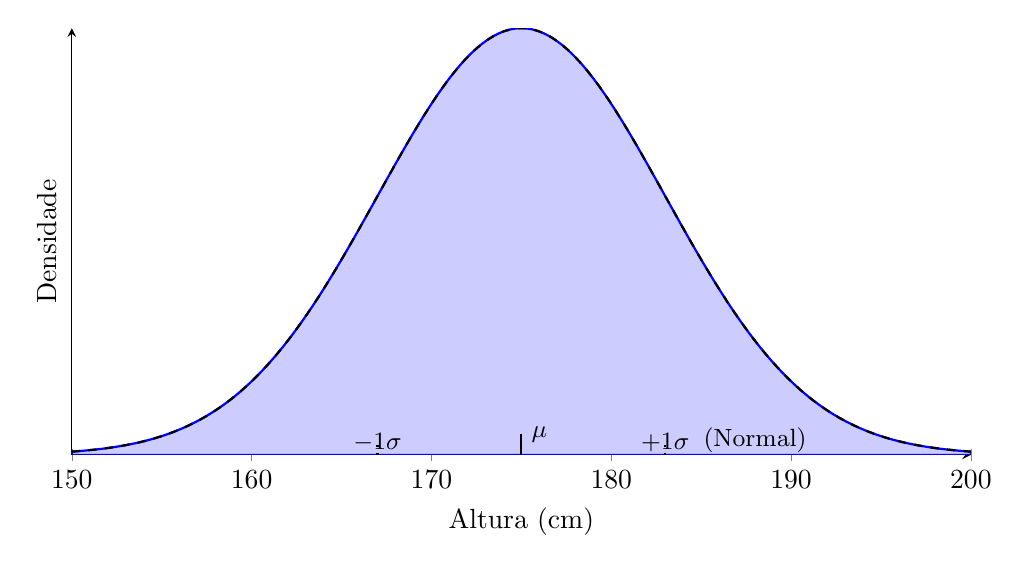
\begin{tikzpicture}
\begin{axis}[
    domain=150:200,
    samples=300,
    axis lines=left,
    xlabel={Altura (cm)},
    ylabel={Densidade},
    width=13cm,
    height=7cm,
    ymin=0,
    xtick={150,160,170,180,190,200},
    ytick=\empty
]
%-----------------------------
% Curva Mesocúrtica (Normal)
%-----------------------------
\addplot[
    thick,
    blue,
    fill=blue!20
]
{exp(-((x-175)^2)/(2*8^2))} \closedcycle;
%-----------------------------
% Curva Normal de Referência
%-----------------------------
\addplot[
    thick,
    black,
    dashed
]
{exp(-((x-175)^2)/(2*8^2))};
%-----------------------------
% Linha da Média
%-----------------------------
\addplot[
    thick,
    black
]
coordinates {(175,0) (175,0.05)};
\node at (axis cs:176,0.048)
{\small $\mu$};
%-----------------------------
% ±1 Desvio-Padrão
%-----------------------------
\addplot[dotted, thick] coordinates {(167,0) (167,0.03)};
\addplot[dotted, thick] coordinates {(183,0) (183,0.03)};
\node at (axis cs:167,0.028) {\small $-1\sigma$};
\node at (axis cs:183,0.028) {\small $+1\sigma$};
% Texto interno
\node at (axis cs:188,0.035)
{\small (Normal)};
\end{axis}
\end{tikzpicture}
\caption{Distribuição mesocúrtica: altura humana segue aproximadamente a curva normal.}
\end{figure}



A altura de adultos tende a formar uma distribuição mesocúrtica, pois os valores se concentram moderadamente ao redor da média (ex.: 175 cm), sem extremos relevantes


%-------------------------------------------------------------------------------%

\newpage
\subsection{Leptocúrtica (mais pontiaguda)}

Em estudos clínicos, a variável glicemia pode apresentar curtose elevada quando:

\begin{itemize}
    \item muitos indivíduos estão próximos do normal (≈100 mg/dL);
    \item poucos pacientes apresentam hiperglicemia severa.
\end{itemize}

Isso gera uma curva com pico alto e caudas pesadas, típica de uma distribuição leptocúrtica. \vskip0.3cm

Exemplo realista de dados (mg/dL)

$$ x = {[90,92,95,100,105,280]} $$

\begin{figure}[H]
\centering
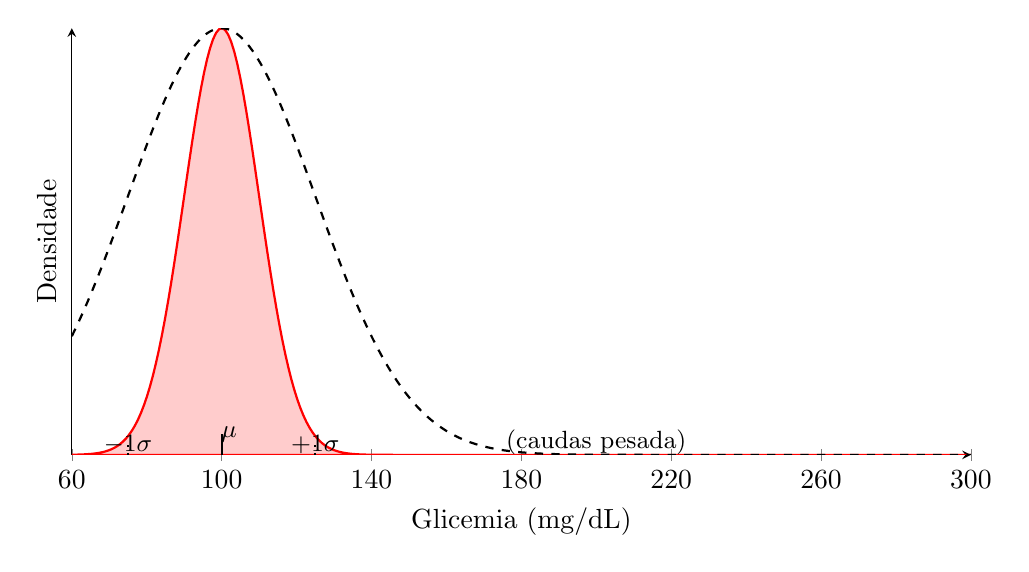
\begin{tikzpicture}
\begin{axis}[
    domain=60:300,
    samples=300,
    axis lines=left,
    xlabel={Glicemia (mg/dL)},
    ylabel={Densidade},
    width=13cm,
    height=7cm,
    ymin=0,
    xtick={60,100,140,180,220,260,300},
    ytick=\empty
]
%-----------------------------
% Curva Leptocúrtica (pico alto)
%-----------------------------
\addplot[
    thick,
    red,
    fill=red!20
]
{exp(-((x-100)^2)/(2*10^2))} \closedcycle;
%-----------------------------
% Curva Normal de Referência
%-----------------------------
\addplot[
    thick,
    black,
    dashed
]
{exp(-((x-100)^2)/(2*25^2))};
%-----------------------------
% Linha da Média
%-----------------------------
\addplot[thick, black]
coordinates {(100,0) (100,0.05)};
\node at (axis cs:102,0.048)
{\small $\mu$};
%-----------------------------
% ±1 Desvio-Padrão
%-----------------------------
\addplot[dotted, thick] coordinates {(75,0) (75,0.025)};
\addplot[dotted, thick] coordinates {(125,0) (125,0.025)};
\node at (axis cs:75,0.023) {\small $-1\sigma$};
\node at (axis cs:125,0.023) {\small $+1\sigma$};
% Texto interno
\node at (axis cs:200,0.03)
{\small (caudas pesada)};

\end{axis}
\end{tikzpicture}
\caption{Distribuição leptocúrtica: glicemia apresenta concentração central e possíveis valores extremos.}
\end{figure}



\newpage
%-------------------------------------------------------------------------------%
\subsection{Platicúrtica (mais achatada)}

O tempo de reação neurológico frequentemente apresenta grande variabilidade, pois depende de fatores como:

\begin{itemize}
    \item Idade;
    \item Fadiga;
    \item Uso de Medicamentos;
    \item Condições Cognitivas;
\end{itemize}


Assim, os valores ficam mais espalhados e a curva se torna achatada, caracterizando uma distribuição platicúrtica. \vskip0.3cm

Exemplo realista de dados (ms)

$$ x = {[180,250,350,500,650]} $$

Os valores são bastante dispersos, reduzindo o pico central.

\begin{figure}[H]
\centering
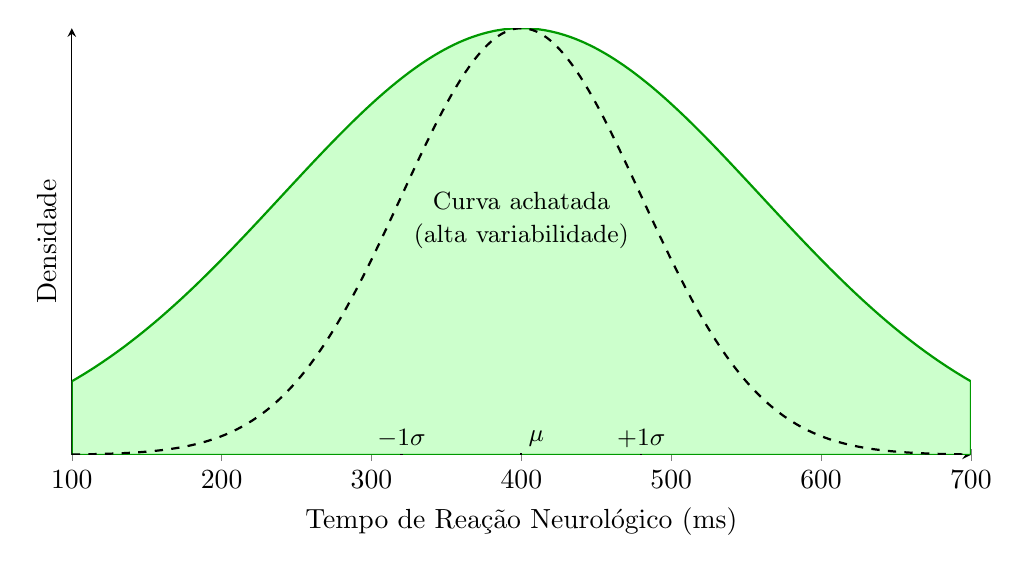
\begin{tikzpicture}
\begin{axis}[
    domain=100:700,
    samples=300,
    axis lines=left,
    xlabel={Tempo de Reação Neurológico (ms)},
    ylabel={Densidade},
    width=13cm,
    height=7cm,
    ymin=0,
    xtick={100,200,300,400,500,600,700},
    ytick=\empty
]

% Curva Platicúrtica
\addplot[
    thick,
    green!60!black,
    fill=green!20
]
{exp(-((x-400)^2)/(2*160^2))} \closedcycle;

% Curva Normal de Referência
\addplot[
    thick,
    black,
    dashed
]
{exp(-((x-400)^2)/(2*80^2))};

% Linha da Média
\addplot[thick, black]
coordinates {(400,0) (400,0.004)};
\node at (axis cs:410,0.038) {\small $\mu$};

% ±1 Desvio-Padrão
\addplot[dotted, thick] coordinates {(320,0) (320,0.002)};
\addplot[dotted, thick] coordinates {(480,0) (480,0.002)};
\node at (axis cs:320,0.038) {\small $-1\sigma$};
\node at (axis cs:480,0.038) {\small $+1\sigma$};

% Texto interno corrigido (NÃO corta mais)
\node[
    align=center,
    text width=4cm
]
at (rel axis cs:0.50,0.55)
{\small Curva achatada\\(alta variabilidade)};

\end{axis}
\end{tikzpicture}
\caption{Distribuição platicúrtica: tempo de reação apresenta grande dispersão entre indivíduos.}
\end{figure}


%-------------------------------------------------------------------------------%